\documentclass[a4paper]{article}
\usepackage[hmargin={30mm,30mm},vmargin={30mm,30mm}]{geometry}


% FONT
\usepackage[T1]{fontenc}
\usepackage{charter}
\usepackage{BOONDOX-calo}
%\usepackage{sectsty}
%\allsectionsfont{\scshape}


% CITATION STYLE
\usepackage{harvard}


% MATHS
\usepackage{euler}
\usepackage{amsmath, amsthm, amssymb, mathtools, stmaryrd}
\usepackage{tikz-cd}
\usepackage{enumerate}
%\usepackage{unicode-math}


% LINE SPACING
\usepackage[parfill]{parskip}
\usepackage[capitalise]{cleveref}
\renewcommand{\baselinestretch}{1.25}


% TODOS
\usepackage[colorinlistoftodos]{todonotes}


% TABLE OF CONTENTS
\usepackage{tocloft}
\renewcommand\contentsname{}
\renewcommand\cftsecfont{}
\renewcommand\cftsecpagefont{}
\setlength\cftbeforesecskip{3pt}
\setcounter{tocdepth}{2}


% THEOREM STYLES
\theoremstyle{definition}
\newtheorem{defn}{Definition}[section]

\newtheorem{theorem}[defn]{Theorem}
\newtheorem*{theorem*}{Theorem}
\newtheorem{prop}[defn]{Proposition}
\newtheorem{lemma}[defn]{Lemma}
\newtheorem{cor}[defn]{Corollary}

\newtheorem{example}[defn]{Example}

\theoremstyle{remark}
\newtheorem{remark}[defn]{Remark}


% NEW ARROWS
\usepackage{stackrel}
\newcommand{\leftrarrows}{\mathrel{\raise.75ex\hbox{\oalign{%
  $\scriptstyle\leftarrow$\cr
  \vrule width0pt height.5ex$\hfil\scriptstyle\relbar$\cr}}}}
\newcommand{\lrightarrows}{\mathrel{\raise.75ex\hbox{\oalign{%
  $\scriptstyle\relbar$\hfil\cr
  $\scriptstyle\vrule width0pt height.5ex\smash\rightarrow$\cr}}}}
\newcommand{\Rrelbar}{\mathrel{\raise.75ex\hbox{\oalign{%
  $\scriptstyle\relbar$\cr
  \vrule width0pt height.5ex$\scriptstyle\relbar$}}}}
\newcommand{\longleftrightarrows}{\leftrarrows\joinrel\Rrelbar\joinrel\lrightarrows}

\makeatletter
\def\leftrightarrowsfill@{\arrowfill@\leftrarrows\Rrelbar\lrightarrows}
\newcommand{\xleftrightarrows}[2][]{\ext@arrow 3399\leftrightarrowsfill@{#1}{#2}}
\makeatother

\usepackage{scalerel}
\newcommand{\simrightarrow}{\mathrel{\ooalign{
     $\to$\cr
     \hidewidth\raise.3em\hbox{$\scaleobj{.7}{\sim}\mkern7mu$}\cr
    }
  }
}

\makeatletter
\newcommand*{\doublerightarrow}[2]{\mathrel{
  \settowidth{\@tempdima}{$\scriptstyle#1$}
  \settowidth{\@tempdimb}{$\scriptstyle#2$}
  \ifdim\@tempdimb>\@tempdima \@tempdima=\@tempdimb\fi
  \mathop{\vcenter{
    \offinterlineskip\ialign{\hbox to\dimexpr\@tempdima+1em{##}\cr
    \rightarrowfill\cr\noalign{\kern.5ex}
    \rightarrowfill\cr}}}\limits^{\!#1}_{\!#2}}}
\newcommand*{\triplerightarrow}[1]{\mathrel{
  \settowidth{\@tempdima}{$\scriptstyle#1$}
  \mathop{\vcenter{
    \offinterlineskip\ialign{\hbox to\dimexpr\@tempdima+1em{##}\cr
    \rightarrowfill\cr\noalign{\kern.5ex}
    \rightarrowfill\cr\noalign{\kern.5ex}
    \rightarrowfill\cr}}}\limits^{\!#1}}}
\makeatother


% CUSTOM COMMANDS
\newcommand{\Exter}{\mathchoice{{\textstyle\bigwedge}}%
    {{\bigwedge}}%
    {{\textstyle\wedge}}%
    {{\scriptstyle\wedge}}}

\newcommand{\grMod}{\ensuremath{\text{-grMod}}}
\newcommand{\Mod}{\ensuremath{\text{-Mod}}}
\newcommand{\dgMod}{\ensuremath{\text{-dgMod}}}
\newcommand{\dgComod}{\ensuremath{\text{-dgCom}}}

\DeclareMathOperator{\Sym}{\text{Sym}}
\DeclareMathOperator{\exterior}{\Exter^\bullet}

\DeclareMathOperator{\coker}{\text{coker}}
\DeclareMathOperator{\img}{\text{im}}
\DeclareMathOperator{\Hom}{\text{Hom}}
\DeclareMathOperator{\Homsh}{\mathcal{H\kern -3pt o\kern -2pt m\kern -1pt}}
\DeclareMathOperator{\Extsh}{\mathcal{E\kern -1pt x\kern -2pt t\kern -1pt}}
\DeclareMathOperator{\cone}{\mathcal{C\kern -2pt o \kern -2pt n \kern -2pt e
\kern -2pt}}
\DeclareMathOperator{\cyl}{\mathcal{C\kern -2pt y \kern -2pt l\kern -2pt}}
\DeclareMathOperator{\Ch}{\mathbf{C}}
\DeclareMathOperator{\kom}{{\mathbf{K}}}
\newcommand{\deri}{\mathbf{D}}

\newcommand{\deritensor}{\ensuremath{\otimes^\mathbf{L}}}

\newcommand{\Proj}{\ensuremath{\text{Proj}}}
\newcommand{\Pn}{\ensuremath{{\mathbb{P}^n}}}
\DeclareMathOperator{\coh}{\mathcal{C\kern -2pt o\kern -2pt h\kern -1pt}}
\DeclareMathOperator{\Qcoh}{\mathcal{Q \kern -2pt c\kern -3pt o\kern -2pt h\kern -1pt}}
\DeclareMathOperator{\sh}{\mathcal{S\kern -2pt h\kern -2pt}}

\newcommand{\gnab}{{\textexclamdown}}

% DOCUMENT
\title{Derived Equivalences in Algebra and Geometry}
\author{Parth Shimpi}
\date{Easter 2022 \\ \vspace{2em}\small{Essay submitted in partial fulfillment of the requirements for \\ Master of
Mathematics degree at the University of Cambridge. \\ 
\vspace{3em}\hrule}}


\begin{document} 
\bibliographystyle{agsm}

\maketitle
\begin{center}
    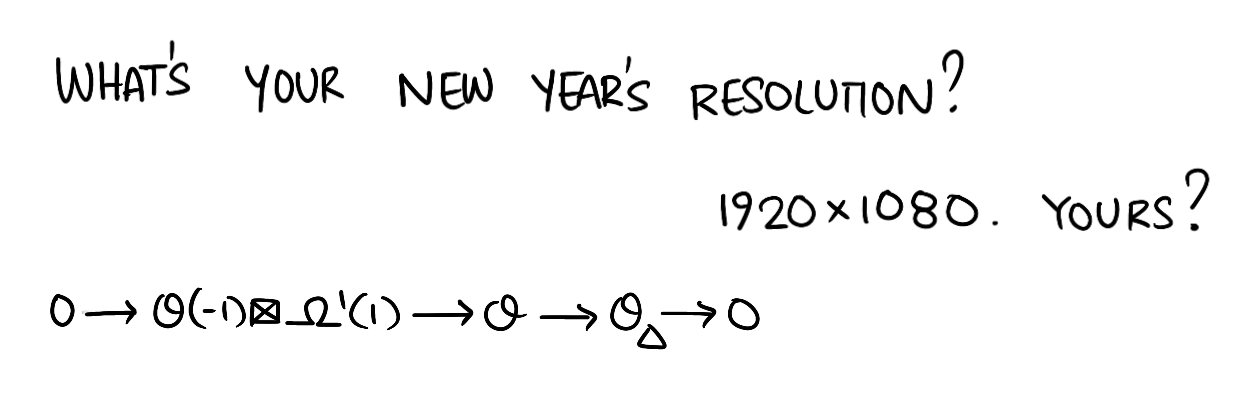
\includegraphics[width=10cm]{head-art.png}
    
    \textit{Both the computer scientist and the mathematician were confused
    \\about why nobody invited them to the party that year.}
\end{center}
\vspace{5em}

\tableofcontents 
\pagebreak

\section*{Introduction}

Fix a field \(k\), and let \(X\) and \(\Xi\) be dual \(k\)-vector spaces of
dimension \(n+1\) with dual bases \((x_i)\) and \((\xi_i)\) respectively. The goal
of this exposition is to examine equivalences of various categories that arise
naturally in this setting from algebro-geometric constructions. In particular,
we look at chain complexes of 
\begin{enumerate}[(i)]
    \item modules over the symmetric algebra \(A:=
        \Sym^\bullet(X)\),
    \item modules over the exterior algebra \(A^!:= \exterior(\Xi)\),
    \item coherent sheaves over \(\Pn := \Proj(\Sym^\bullet (X))\), the
        projectivisation of \(\Xi\).
\end{enumerate}

To set the stage, we examine an algorithm to functorially obtain free
resolutions of \(k[x]\)-modules.

\begin{example}\label{setstage}
In the simplest case when \(X, \Xi\) are one-dimensional, the data of a module
over \(A = k[x]\) involves a \(k\)-vector space \(M\) with a map
\(M\xrightarrow{x} M\) which can be seen as a complex \(F(M)\) of
\(k\)-vector spaces with differential \(d\) of degree \(1\). In other words, the
underlying vector space \(F(M) = M\oplus M\) is a module over the graded algebra
\(A^! = k[\xi]/(\xi^2)\), where the map \(F(M)\xrightarrow{\xi} F(M)\) is given by
\[\begin{tikzcd}[column sep = tiny, row sep = large]
    M \arrow[rrd, "1"] & \oplus &  M \arrow[rrd] & \oplus & 0\\ 
    M & \oplus & M & \oplus & 0 
\end{tikzcd}.\]
Consider the complex \(G(F(M))\) of \(A\)-modules
\[\cdots \rightarrow 0 \rightarrow M\otimes_k A
\xrightarrow{ d\otimes 1 + \xi \otimes x} M\otimes_k A \rightarrow 0 \rightarrow
\cdots ,\]
concentrated in degrees \(-1\) and \(0\). This can be seen as the complex \(F(M)\otimes_k A\), but the differential has been
`twisted' to remember the \(A^!\)-action. This complex is exact everywhere
except in degree \(0\), where it has cohomology \(M\). Since the modules
appearing in it are free, we have recovered a free resolution of \(M\).
Moreover, the construction is functorial i.e.\ an \(A\)-module homomorphism
\(M\rightarrow M'\) naturally induces a chain map \(G(F(M))\rightarrow
G(F(M'))\). 
\end{example}

This is the first example of what may be called \textit{Koszul duality}, a broad
term encompassing various equivalences across algebra, geometry, and representation
theory. The duality between symmetric and exterior algebras over finite
dimensional vector spaces was first studied by
\citeasnoun{bernstein_algebraic_1978}, who exhibit an adjunction between the
categories of complexes of graded modules over \(A\) and \(A^!\).  
\begin{theorem*}
    There are adjoint functors
    \[ \Ch(A\grMod) \xleftrightarrows[F]{G} \Ch(A^!\grMod)\]
    such that any complex \(\mathbf{M}\) of graded
    \(A\)-modules has free resolution \(GF(\mathbf{M})\), and any complex
    \(\mathbf{N}\) of graded \(A^!\)-modules has injective resolution
    \(FG(\mathbf{N})\). 
\end{theorem*}
In \cref{sec-BGG}, we look at \possessivecite{eisenbud_sheaf_2003}
treatment of the Bernstein-Gel'fand-Gel'fand (BGG) correspondence described
above. In particular, we have a functorial method to obtain resolutions-- this
allows for a succinct proof of Hilbert's theorem on syzygies which we discuss as an
application. 

To formulate a more precise result on Koszul duality, we need to
employ the machinery of Verdier's \textit{derived categories}. We begin by
describing this and related constructions from
homological algebra in \cref{sec-trianglecat}. In particular, rings and schemes
have associated derived categories whose objects are chain complexes of modules
and sheaves respectively, considered up to \textit{quasi-isomorphism} (i.e.\
chain maps that preserve homology). Thus, for
instance, a sheaf and its injective resolution are the same object in the
derived category. This provides a framework which lets us make clean statements
about cohomology, and as we see, is in fact an enhancement of the classical
notion of cohomology. 

Certain schemes such as Grassmannians have a nice description of the associated
derived category. In \cref{sec-cohPn} we prove the celebrated theorem of
\citeasnoun{beilinson_coherent_1978} which asserts that the derived category of
\Pn\ is built from \(n+1\) line bundles.

\begin{theorem*}
    The bounded derived category of \(\mathbb{P}^n\) is generated by the set 
    \(\{\mathscr{O}_{\Pn}, \mathscr{O}_{\Pn}(-1),...,\mathscr{O}_{\Pn}(-n)\)\}.
\end{theorem*}

For instance, every coherent sheaf \(\mathscr{A}\) on \(\Pn\)
admits a resolution by finite direct sums of the line bundles
\(\mathscr{O}(-i)\) (\(0\leq i \leq n\)). The use of Koszul resolutions and
Fourier-Mukai transforms in Beilinson's proof gives an algorithm which lets us
directly compute the explicit form of this resolution-- in particular we show
that this depends only on the cohomology of a few twists of \(\mathscr{A}\).
\citeasnoun{eisenbud_sheaf_2003} uses the BGG functors to reconstruct this
resolution, and comparing the two constructions provides an algorithm to compute
sheaf cohomology.

\paragraph{Acknowledgement.} The author is grateful to Dhruv Ranganathan for
introducing them to derived categories; to Ismael Sierra del Rio for providing
various perspectives on Koszul duality; and to Ian Grojnowski for guidance
through the essay.

\section{Categories of complexes}\label{sec-trianglecat}

We set up the basic framework of homological algebra and derived
categories necessary to formulate results in later sections. The material is
largely taken from \citeasnoun{weibel_introduction_2003} and the initial
chapters of \citeasnoun{huybrechts_fourier-mukai_2006}, with heuristics taken
from \citeasnoun{thomas_derived_2001}.

A category \(\mathfrak{A}\) is \textit{additive} if each hom-set
\(\Hom_\mathfrak{A}(A,B)\) has the structure of an abelian group such that
composition distributes over addition, \(\mathfrak{A}\) has finite products, and
there is an object \(0\in \mathfrak{A}\) such that for any \(A\in
\mathfrak{A}\), \(\Hom_\mathfrak{A}(A,0)\) and \(\Hom_\mathfrak{A}(0,A)\) are
the trivial group. In this setting we can make sense of the kernel and cokernel
morphisms, which are defined using their usual universal properties.

We say an additive category \(\mathfrak{A}\) is \textit{abelian} if every
morphism in \(\mathfrak{A}\) has a kernel and cokernel, and these behave as
expected (i.e.\ every monomorphism is the kernel of its cokernel and every
epimorphism is the cokernel of its kernel). Abelian categories provide the right
framework to talk about exact sequences and cohomology, which is the essence of
homological algebra. The prototypical example of an abelian category is the
category \(R\Mod\) of (left) modules on a ring \(R\). 

All the abelian categories occuring in this exposition come from categories of
modules over a ring, or sheaves on a topological space. In both the cases, the
notions of kernel, cokernel, image, exact sequence, and cohomology are the usual
ones.

\begin{example}[Endomorphism rings] \label{ring-additive}
    For any object \(A\) in an additive category \(\mathfrak{A}\), the group
    \(\Hom_\mathfrak{A}(A,A)\) naturally has the structure of a unital ring, where
    multiplication is given by composition. Then any unital ring \(R\) can be
    seen as an additive category with a single non-zero object \(\ast\), such
    that \(\Hom_\mathfrak{A}(\ast,\ast)\cong R\). Thus rings are two-object
    abelian categories!  
\end{example}

\begin{example}[Chain complexes] 
    A \textit{chain complex} \(\mathbf{A}\) in an additive category
    \(\mathfrak{A}\) is a sequence of objects \((A^i)_{i\in\mathbb{Z}}\) and
    morphisms \(d^i:A^i\rightarrow A^{i+1}\) (called the \textit{differentials})
    such that the compositions \(d^i\circ d^{i-1}\) are all \(0\). We say the
    object \(A^i\) sits in differential degree \(i\). If all but finitely many
    \(A^i\)s are the zero object, then the chain complex is said to be
    \textit{bounded}.

    A \textit{chain-map} \(f: \mathbf{A} \rightarrow
    \mathbf{B}\) is a sequence \((f^i:A^i\rightarrow B^i)_{i\in \mathbb{Z}}\) of
    morphisms in \(\mathfrak{A}\) such that \({f^{i+1}\circ d^i = d^i \circ
    f^i}\) for all \(i\). Then associated to \(\mathfrak{A}\) is a category
    \(\Ch(\mathfrak{A})\) whose objects are chain complexes in \(\mathfrak{A}\),
    and morphisms are chain-maps. This is naturally an abelian category, where
    the zero object is the complex which has \(0\) in every differential degree.
    Write \(\Ch^b(\mathfrak{A})\), \(\Ch^+(\mathfrak{A})\), and
    \(\Ch^-(\mathfrak{A})\) for the full subcategories whose objects are
    bounded complexes, complexes bounded below, and complexes bounded
    above respectively. These are again examples of abelian categories.
\end{example}

The notions of additive and abelian categories come naturally with notions of
functors which preserve the additional structures-- these are called
\textit{additive} and \textit{exact} functors.

\begin{defn}
    A functor \(F:\mathfrak{A}\rightarrow \mathfrak{B}\) between additive
    categories is called an \textit{additive functor} if the maps \(F:
    \Hom_\mathfrak{A}(A,B)\rightarrow \Hom_{\mathfrak{B}}(FA,FB)\) are group
    homomorphisms. We say \(F\) is \textit{exact} if, in addition, it sends
    short exact sequences to short exact sequences.
\end{defn}

\begin{example}[Additive functors on chain complexes] Let \(\mathfrak{A}\)
    be any additive category.
    \begin{enumerate} 
        \item There is a natural inclusion \(\mathfrak{A}\rightarrow
            \Ch(\mathfrak{A})\) which sends an object \(A\) to the chain complex
            \(A^\bullet\) where \(A^0=A\), and \(A^i=0\) for \(i\neq 0\).
            This is an exact functor, identifying \(\mathfrak{A}\) as a
            full abelian subcategory of \(\Ch(\mathfrak{A})\).  
        \item Given \(A^\bullet\in \Ch(\mathfrak{A})\), we define the
            \textit{translate by \(1\)} of \(A^\bullet\) to be the chain complex
            \(A^\bullet[1]\), which has \(A^{i+1},-d^{i+1}\) in degree \(i\).
            This defines an exact functor \([1]:\mathfrak{A}\rightarrow
            \mathfrak{A}\) which is an equivalence of categories. Write \([i]\)
            for the \(i\)-fold composition of \([1]\) with itself, and \([-i]\)
            for the functor inverse to \([i]\).
        \item For any \(i\in \mathbf{Z}\), the functor \(H^i:
            \Ch(\mathfrak{A})\rightarrow \mathfrak{A}\) which sends a complex
            \(\mathfrak{A}\) to its cohomology at \(A^i\) is an additive
            functor. We say \(\mathbf{A}\) is \textit{exact at \(A^i\)} if
            \(H^i(\mathbf{A})=0\). The complex is \textit{acyclic} (or
            \textit{exact}) if it is exact at every \(A^i\).
    \end{enumerate}
\end{example}

\subsection{Bicomplexes}

If \(\mathfrak{A}\) is an abelian category, then so is \(\Ch(\mathfrak{A})\) so
we can construct a category \(\Ch(\Ch(\mathfrak{A}))\) whose objects are
\textit{bicomplexes} of the form
\begin{equation}\label{bicomplex}\begin{tikzcd}
    \vdots       &        & \vdots & \vdots &   \\
    \mathbf{A}^{p+1}:\arrow[u] & \cdots\arrow[r] & A^{p+1, q}\arrow[u] \arrow[r] & A^{p+1, q+1} \arrow[r] \arrow[u] & \cdots \\
    \mathbf{A}^p:\arrow[u]     & \cdots\arrow[r] & A^{p, q}\arrow[u]\arrow[r]
                               & A^{p, q+1}\arrow[u] \arrow[r]   & \cdots \\
    \vdots\arrow[u]            &        & \vdots\arrow[u] & \vdots\arrow[u] &   
\end{tikzcd}.\end{equation}
where all the squares commute. Here the horizontal differentials (which we write
\(d_{>}\) for) come from the internal differentials of the chain complexes
\(\mathbf{A}^i\in \Ch(\mathfrak{A})\), while the vertical differentials (which
we write \(d_\wedge\) for) come from the differentials of the complex in
\(\Ch(\Ch(\mathfrak{A}))\). 

Such bicomplexes have an associated \textit{total (direct sum) complex} in
\(\Ch(\mathfrak{A})\), given by 
\[ \cdots \rightarrow \bigoplus_{p+q=i-1}A^{p,q} \longrightarrow
\bigoplus_{p+q=i}A^{p,q} \rightarrow \cdots\]
where the differential sends \(a\in A^{p,q}\) to \(d_\wedge(a) + (-1)^i
d_>(a)\). If direct products are taken instead of direct sums, we have the total
direct product complex. In the case of bounded bicomplexes the two notions
coincide.

\begin{example}
    Given two chain complexes \(\mathbf{A}, \mathbf{B}\in R\Mod\) for some ring
    \(R\), there is an associated bicomplex \(\mathbf{A}\otimes_R \mathbf{B}\)
    given in degree \((p,q)\) by \(A^p\otimes_R B^q\). Then the \textit{total tensor
    product complex} \(\text{Tot}(\mathbf{A}\otimes_R \mathbf{B})\) is the total
    direct sum complex of this bicomplex. 

    Likewise, defining the bicomplex \(\Hom_R(\mathbf{A},\mathbf{B})\) in degree
    \((p,q)\) by \(\Hom_R(A^p,B^q)\). The \textit{total Hom complex}
    \(\text{Tot} (\Hom_R(\mathbf{A},\mathbf{B}))\) is the total direct
    product complex of this bicomplex. The
    usual \({\otimes-\Hom}\) adjunction extends to
    these total complexes, the details can be
    found in \citeasnoun{weibel_introduction_2003}.
\end{example} 

\subsubsection{Spectral sequences.} 
Often, one is interested in the cohomology of the total complex associated to
a bicomplex. \textit{Spectral sequences} provide a bookkeeping tool for this
purpose, and often allow us to extract the cohomology of the bicomplex from the
cohomologies of the rows or columns. We will only deal with spectral sequences
associated to bicomplexes of modules, so the category \(\mathfrak{A}\) is a
module category for the purposes of this section.

The \textit{spectral sequence (starting with horizontal cohomology)}
\(\mathbf{E}\) of a bicomplex \eqref{bicomplex} is a sequence of \textit{pages}
\(\mathbf{E}_i\), where each page has objects of \(\mathfrak{A}\) arranged in a
grid \(E^{p,q}_i\) with specified morphisms which we now describe. The zeroth
page is given by forgetting the vertical differentials in \eqref{bicomplex}, as
\[\begin{tikzcd}[row sep=tiny]
    & \vdots & \vdots & \\
    \cdots \arrow[r] & A^{p+1,q} \arrow[r] & A^{p+1,q+1} \arrow[r] &\cdots \\
    \cdots \arrow[r] & A^{p,q} \arrow[r] & A^{p,q+1} \arrow[r] &\cdots  \\
    & \vdots & \vdots & \\
\end{tikzcd}.\]
The objects in the first page will be the cohomologies of the sequences in
\(\mathbf{E}_0\), with maps between them induced by the vertical differentials
\(d_\wedge\).
\[\begin{tikzcd}[column sep = tiny] 
    &\vdots &\vdots & \\
    \cdots & H^q(\mathbf{A}^{p+1}) \arrow[u] &   H^{q+1}(\mathbf{A}^{p+1}) \arrow[u]
           & \cdots \\
    \cdots & H^q(\mathbf{A}^{p}) \arrow[u] &   H^{q+1}(\mathbf{A}^{p}) \arrow[u]
           & \cdots \\
           &\vdots\arrow[u] &\vdots\arrow[u] & 
\end{tikzcd}.\]
The subsequent pages are defined likewise-- in particular, the morphisms on the
\(i\)th page go from \(E_i^{p,q}\) to \(E_i^{p+i,q-i-1}\) and the compositions
of the morphisms, whenever defined, are zero (so that the \(i\)th page contains a
sequence of complexes.) The objects on \(\mathbf{E}_i\) are then the
cohomologies of the complexes on \(\mathbf{E}_{i-1}\), and the morphisms described
above are induced from the previous pages. 

All the spectral sequences we consider in this exposition are \textit{regular},
i.e.\ there is an \(r\geq 2\) such that the morphisms on every page after
\(\mathbf{E}_r\) are zero. In this case, we have \(E^{p,q}_r = E^{p,q}_{r+1} =
... = E^{p,q}_\infty\) for some object \(E^{p,q}_\infty \in \mathfrak{A}\).

\begin{defn}
    Given a sequence \(H^\bullet=(..., H^{-1},H^0,H^1,...)\) of objects in
    \(\mathfrak{A}\), we say a (regular) spectral sequence \(\mathbf{E}\)
    \textit{converges weakly} to \(H^\bullet\) if for every \(i\) there exists a
    filtration 
    \[\cdots \subseteq F^2H^i \subseteq F^{1}H^i \subseteq F^0H^i =
    H^i \] such that for every \(p\geq 0\) and for every \(q\), we have 
    \[\frac{F^pH^{p+q}}{F^{p+1}H^{p+q}} \cong E^{p,q}_\infty.\]
    If in addition for all \(i\) we have \(\bigcap_pF^pH^i= 0\) and \(H^i =
    \lim_p H^i/F^pH^i\), then we say the spectral sequence \textit{converges} to
    \(H^\bullet\).
\end{defn}

For a general bicomplex as in \eqref{bicomplex}, not much can be said about
convergence of the spectral sequence. However, if the bicomplex is
\textit{bounded} i.e.\ for every \(i\) there are only finitely many non-zero
\(A^{p,q}\) with \(p+q=i\) then we have the following result.
\pagebreak

\begin{prop}\label{spectral-convergence}
    If the bicomplex \eqref{bicomplex} is bounded, then the spectral sequence
    \(\mathbf{E}\) converges to the sequence \(H^\bullet\) where \(H^i\) is the
    \(i\)th homology object of the total (direct sum) complex of the bicomplex.
    \begin{proof}
        See Lemma 12.25.3 of \citeasnoun{stacks-project}.
    \end{proof}
\end{prop}

\subsection{Three abelian categories}

Before proceeding with more constructions from homological algebra, we describe
the three abelian categories central to this exposition-- these are the module
categories of the symmetric and exterior algebra, and the category of coherent
sheaves on \(\Pn\). These are defined in the usual way, but we record the
constructions involved for completeness of exposition, and to set conventions. 

Let \(k\), \(X\), and \(\Xi\) be as in the introduction.

\subsubsection{Symmetric and exterior algebras.} 

\begin{defn} 
    Given an \(n+1\)-dimensional \(k\)-vector space \(V\), the \textit{tensor
    algebra} is the \(k\)-vector space 
    \[ T(V) = k \oplus \bigoplus_{i\geq 1}(\underbrace{V\otimes_k V\otimes_k ...
    \otimes_k V}_{i\text{ times}})\] 
    with a product \(\nabla: T(V)\otimes T(V) \rightarrow T(V)\) induced by the
    natural identifications \(V^{\otimes i}\otimes V^{\otimes j} \simrightarrow
    V^{\otimes(i+j)}\). This is an associative algebra with a natural
    \(\mathbb{Z}_{\geq 0}\)-grading. 

    The \textit{symmetric algebra} \(\Sym^\bullet(V)\) and the \textit{exterior
    algebra} \(\exterior(V)\) are then the graded algebras defined as quotients
    of \(T(V)\) by certain two-sided ideals, namely 
    \[\Sym^\bullet(V) = \frac{T(V)}{(x\otimes y - y\otimes x \;|\; x,y\in V)},
    \qquad \exterior(V) = \frac{T(V)}{(x\otimes x \;|\; x\in V)}.\] 
    Since the ideals are generated by homogeneous elements, these algebras
    inherit gradings from \(T(V)\).
\end{defn}

We continue to use \(\nabla\) for the product morphism on either algebra,
though the corresponding bilinear map on \(\exterior{V}\) is often written
\(\wedge\).

\begin{remark} 
    We can repeat the above constructions in the category of \(R\)-modules for
    any ring \(R\). In this case, we write \(T_R(M),\; \Sym^\bullet_R(M),\;
    \Lambda^\bullet_R(M)\) respectively for the tensor, symmetric, and exterior
    algebras over \(M\in R\Mod\). In particular,
    \[ T(M) = R \oplus \bigoplus_{i\geq 1}(\underbrace{M\otimes_R M\otimes_R ...
    \otimes_R M}_{i\text{ times}}).\]
\end{remark}

Since we are primarily concerned with the algebras \(A=\Sym^\bullet(X)\) and
\(A^!=\exterior(\Xi)\), we redefine the grading on \(A^!\) as
\(A^!_{-i}=\Lambda^i \Xi\). This amounts to a change of sign from the usual
grading, but the convention ensures that the dual vector spaces \(X\) and
\(\Xi\) lie in degrees \(1\) and \(-1\) in their respective algebras.

\paragraph{Graded modules.} A graded \(A\)-module is a \(\mathbb{Z}\)-graded
\(k\)-vector space \(\mathbf{M} = \oplus_i M_i\) with an \(A\)-module structure
such that \(A_iM_j \subseteq M_{i+j}\). For any \(i\), we say the elements of
\(M_i\) are homogeneous of degree \(i\). A morphism of graded modules then is an
\(A\)-module homomorphism that preserves the degree of homogeneous elements.
Define the category \(A\grMod\) to have  finitely genered graded \(A\)-modules
as its objects, and graded module homomorphisms as the morphisms. This is an
abelian category.

The abelian category \(A^!\grMod\) is defined likewise, with objects being
finitely generated graded \(A^!\)-modules.

\subsubsection{The exterior coalgebra}
\label{subsubsec-exteriorcoalgebra}

The \textit{exterior coalgebra} on \(\Xi\) is defined as the linear dual of
\(A^!\), written \(A^\gnab := \Hom_k(A^!, k)\). \(A^\gnab\) has the
\(\mathbb{Z}\)-grading \(A^\gnab_i=\Hom_k(A^!_{-i}, k)\) and is naturally an
\(A^!\)-module via \[a \cdot f(a') = (-1)^{\text{deg}\, a} f(a\wedge a')\]
whenever \(a\in A^!\) is homogeneous, and \(f\in \Hom(A^!,k)\). 

For any vector space \(N\), there is the natural isomorphism of
\(A^!\)-modules \({\Hom_{k}(A^!, N)\cong A^\gnab \otimes_k N}.\)  

Choosing a basis \(x_i\) for \(X\) fixes an isomorphism \(X\cong\Hom_k(\Xi,
k)=A^\gnab_1\), which can be extended to get the isomorphism of graded \(k\)-vector
spaces
\[A^\gnab = \bigoplus_i \Hom_k(\Lambda^i\Xi, k) \cong \bigoplus_i \Lambda^i X =
\exterior(X).\] 
In particular, \(X\) is a subspace of both \(A^\gnab\) and \(A\). This
observation is essential in defining the Koszul duality functors, so we write
\(\tau:A^\gnab \rightarrow A\) for the \(k\)-linear map which identifies the
subspaces of \(A^\gnab\) and \(A\) corresponding to \(X\), and is \(0\) elsewhere. 

\paragraph{The coproduct on \(A^\gnab\).}
Being the linear dual of a finite dimensional algebra, \(A^\gnab\) has a natural
(coassociative counital) coalgebra structure which comes from dualising the
(associative unital) product \({\nabla: A^!\otimes_k A^!\rightarrow A^!}\). This
is called the \textit{shuffle coproduct}, and it is helpful to have an explicit
description of it which we now describe. 

Given a collection of indices \(\underline{\alpha}=\{\alpha_1\,<\,
...\,<\,\alpha_i\}\subseteq \{0,...,n\}\), write \(x_{\underline{\alpha}}\) for the
standard basis element of \(A^\gnab\) given by \({x_{\alpha_1}\wedge
x_{\alpha_2} \wedge ... \wedge x_{\alpha_i}}\) (in particular,
\(x_\emptyset = 1\)). The vector \(\xi_{\underline{\alpha}}\) is defined
similarly. We say a tuple \((\underline{\beta}, \underline{\beta'})\) of subsets
is a \textit{break} of \(\underline{\alpha}\) if \((\beta_1\,<...<\,\beta_p,
\beta'_1\,<...<\,\beta'_q)\) is a permutation of \((\alpha_1\,<...<\,
\alpha_i)\) (in other words, \(\underline{\alpha} = \underline{\beta} \sqcup
\underline{\beta'}\)). The \textit{sign} of this break, written \(\langle
\underline{\beta}, \underline{\beta'}\rangle\), is defined to be the sign of the
corresponding permutation. Thus we have have 
\[\nabla(x_{\underline{\beta}} \otimes
    x_{\underline{\beta'}})=x_{\underline{\beta}} \wedge
    x_{\underline{\beta'}}=\langle \underline{\beta}, \underline{\beta'}\rangle
\, x_{\underline{\alpha}}.\] 
This allows us to write the coproduct on \(A^\gnab\) as 
\[\Delta(x_{\underline{\alpha}}) =
    \smashoperator[r]{\sum\limits_{(\underline{\beta},\underline{\beta'})\in
    \text{br}(\underline{\alpha})}} \langle \underline{\beta},
\underline{\beta'}\rangle \, x_{\underline{\beta}} \otimes
x_{\underline{\beta'}}\]
where \(\text{br}(\underline{\alpha})\) is the set of all breaks of
\(\underline{\alpha}\).  Recalling that \(A^\gnab\otimes_k A^\gnab\) is
\(\mathbb{Z}\)-graded with \(\bigoplus_{p+q=i}A^\gnab_p\otimes A^\gnab_q\) in
degree \(i\), we observe that the map \(\Delta\) respects grading hence
\(A^\gnab\) is a \textit{graded coalgebra}.

\subsubsection{Graded chain complexes}
\label{subsec-chaincomp}

Objects of \(\Ch(A\grMod)\) are chain complexes of graded \(A\)-modules in
which the differentials are morphisms in \(A\grMod\) (i.e.\ \(A\)-module
homomorphisms which preserve degree). Such an object can be viewed as a
\(\mathbb{Z}^2\)-graded \(k\)-vector space \(\mathbf{M}=\bigoplus_{i,j}M^i_j\)
with an endomorphism \(d\) (the differential) such that 
\begin{enumerate}
    \item \(d\circ d=0\), 
    \item \(d\) has degree \((1,0)\) i.e.\ \(d(M^i_j)\subseteq M^{i+1}_j\),
        and
    \item for each \(i\in \mathbb{Z}\), \(M^i_\bullet = \bigoplus_{j}
        M^i_j\) is a graded \(A\)-module.  
\end{enumerate} 
Likewise, an object \(\mathbf{N}\in \Ch(A^!\grMod)\) can be seen as a
\(\mathbb{Z}^2\)-graded \(k\)-vector space \(\oplus_{i,j}N^i_j\) with a
differential \(\partial\) of degree \((1,0)\). We shall use the two viewpoints
on interchangeably, switching between them whenever convenient to provide a
clearer picture. In particular, the ability to view a complex as a single module
with additional structure allows for cleaner definitions and proofs, see for
instance \cref{adjunction}.

For a chain complex \(\mathbf{M}=\bigoplus_{i,j}M^i_j\), we say the lower
indices denote the \textit{internal} (or \textit{Adam's}) grading, while the
upper indices denote the \textit{differential} (or \textit{cohomological})
degree.  We use `\(\langle\cdot\rangle\)' to denote shifts in Adam's gradings,
continuing to use `\([\cdot]\)' to denote shifts in differential gradings.  Thus
for example we have \(\mathbf{M}\langle q \rangle^i_j = M^i_{q+j}\).

\subsubsection{Coherent sheaves}

The details of all the constructions described in this section can be found in
Sections II.5 and II.8 of \citeasnoun{hartshorne_algebraic_2008}.

For any scheme \(\mathbf{X}\), the category \(\sh\mathbf{X}\) of sheaves on
\(\mathbf{X}\) is abelian with the usual notions of kernel and cokernel.
If the scheme \(\mathbf{X}\) is noetherian, then the
(co)kernel of a morphism of coherent sheaves is coherent. In this case, the category
\(\coh\mathbf{X}\) whose objects are coherent sheaves of
\(\mathscr{O}_\mathbf{X}\)-modules is abelian. 

The category \(\coh\mathbf{X}\) supports an additional operation, the tensor
product \(\otimes\). The tensor product of coherent sheaves will always be over
the structure sheaf, unless otherwise specified. Given a coherent sheaf
\(\mathscr{E}\), we can then define the sheaves of algebras \(T\mathscr{E}\),
\(\Sym \mathscr{E}\), and \(\Exter^\bullet \mathscr{E}\) as coming from
the presheaves which assign to an open set \(U\subset \mathbf{X}\) the
corresponding tensor operation applied to \(\mathscr{E}(U)\) as an
\(\mathscr{O}_\mathbf{X}(U)\)-module.

If \(\,\mathbf{X}\xrightarrow{\;f\;} \mathbf{Y}\,\) is a morphism of noetherian
schemes, then the \textit{pullback} of a coherent sheaf on \(\mathbf{Y}\)
is again coherent. This gives an additive functor \[f^\ast:
\coh\mathbf{Y}\longrightarrow \coh\mathbf{X}.\] 
The pullback functor commutes with the various tensor operations described above.

\paragraph{Sheaves on \Pn.} The \textit{projectivisation} of \(\Xi\) is the
\(k\)-scheme defined as \(\Pn = \Proj(\Sym (\Xi^\vee))\). Since
\(\Sym(\Xi^\vee)=A\) is the polynomial algebra on \(n+1\) variables, we see that
\(\Pn\) is the usual projective \(n\)-space over \(\text{Spec}(k)\). This is a
noetherian scheme, and so \(\coh\Pn\) is an abelian category.

Serre gives a correspondence between \(A\grMod\) and
\(\coh\Pn\) using a construction similar to \(\Proj\), called the
`sheafification' of graded modules. This correspondence is functorial, but
\textit{not} an equivalence of categories. Indeed, much of \cref{sec-cohPn} is
dedicated to obtaining a precise formulation of the equivalence between coherent
sheaves on \(\Pn\) and finitely generated graded \(A\)-modules.

In particular, the module \(A\in A\grMod\) corresponds to the structure sheaf
\(\mathscr{O}_\Pn\). Since \(\Pn\) is central to the exposition, we omit the
subscript \(\Pn\) unless there is a possibility of confusion-- thus writing
\(\mathscr{O}\) for the structure sheaf.

The invertible sheaf \(\mathscr{O}(i)\) is defined as the sheafification of
the graded module \(A\langle i \rangle\). In particular, the global sections of
\(\mathscr{O}(i)\) correspond to degree \(i\) polynomials. The various sheaves
\(\mathscr{O}(i)\) form an abelian group under \(\otimes\), there being natural
isomorphisms \(\mathscr{O}(i)\otimes \mathscr{O}(j)\cong \mathscr{O}(i+j).\)
Note that tensor products of sheaves are always taken over the structure
sheaf. 

For any sheaf \({\mathscr{E}\in \coh\Pn}\), its \(i\)th \textit{twist} is defined by
\(\mathscr{E}(i)= \mathscr{E}\otimes \mathscr{O}(i).\) Since the sheaves
\(\mathscr{O}(i)\) are flat, taking the \(i\)th twist is an exact functor.

The \textit{cotangent sheaf} \(\Omega\) and the \textit{tangent sheaf}
\(\mathscr{T}=\Homsh(\Omega, \mathscr{O})\) are locally free sheaves of rank
\(n\) which fit in dual exact sequences given by
\begin{equation} \label{eulerexactsequence}
    0\rightarrow \Omega \rightarrow \mathscr{O}(-1)^{\oplus(n+1)} \rightarrow
    \mathscr{O}\rightarrow 0, \qquad
    0\rightarrow \mathscr{O}\rightarrow \mathscr{O}(1)^{\oplus(n+1)}\rightarrow
    \mathscr{T}\rightarrow 0.
\end{equation}
These are called the \textit{Euler exact sequences}, and form our primary means
of getting hold of the sheaves. In particular, \(\Omega\) corresponds to the
graded module given by the kernel of 
\[A^{n+1}\langle -1 \rangle\longrightarrow A; \qquad (a_0,...,a_n)\longmapsto
a_0x_0+...+a_nx_n.\]

\subsection{Homotopy and Derived categories}

We return to our discussion of homological algebra, to build the framework of
\textit{triangulated categories} and the derived category. Before describing
these, we provide some motivation as to why we construct them by first reviewing
how homological algebra is typically used to find invariants in mathematics.

Given a category \(\mathfrak{C}\), we choose for each
\(X\in \mathfrak{C}\) a complex \(\Phi(X)\in\Ch(\mathfrak{A})\) for some abelian
category \(\mathfrak{A}\). Then the compositions \(H^i\circ \Phi:
\mathfrak{C}\rightarrow \mathfrak{A}\) allow us to assign a sequence of
\(\mathfrak{A}\)-objects associated to \(X\), and this assignment (in the good
cases) is functorial. The following examples illustrate this.
\begin{enumerate}
    \item Consider the category \(\mathcal{S\kern -2pt i \kern -2pt
        m \kern -2pt p\kern -2pt}\) of simplicial complexes (in the sense of
        algebraic topology), and the functor \(F:\mathcal{S\kern -2pt i \kern
        -2pt m \kern -2pt p\kern -2pt}\rightarrow \mathbb{Z}\Mod\) which
        associates to a simplicial complex \(\mathbf{X}\in \mathcal{S\kern -2pt
        i \kern -2pt m \kern -2pt p\kern -2pt} \) the chain complex
        \(F(\mathbf{X})\) of abelian groups where the group in degree \(-i\) is
        generated by \(i\)-simplices, and the differentials are boundary maps.
        If \(\mathcal{T\kern -3pt r}\) is the category of triangulable
        topological spaces, then we can choose a map \(\Phi: \mathcal{T\kern
        -3pt r}\rightarrow \mathcal{S\kern -2pt
        i \kern -2pt m \kern -2pt p\kern -2pt}\) which associates to each
        \(\mathbf{X}\in \mathcal{T\kern -3pt r}\) a simplicial complex which is
        its triangulation. The \(i\)th \textit{simplicial homology} of
        \(\mathbf{X}\) is defined as \(H^{-i}(F(\Phi(\mathbf{X})))\).

    \item For a ring \(R\), let \(\Ch^-_\text{free}(R\Mod)\) be the full
        subcategory of \(\Ch^-(R\Mod)\) whose objects are complexes of
        free \(R\)-modules. Choose for each \(M\in R\Mod\), choose a complex
        \({\Phi(M)\in \Ch^-_\text{free}(R\Mod)}\) such that \(\Phi(M)\) is exact
        in non-zero degrees and has \(H^0(\Phi(M))=M\).  Then for a fixed
        \(R\)-module \(M\), we define the \(i\)th Ext functor by
        \(\text{Ext}^i_R(M,-)=H^{-i}\circ \Hom_R(M,-)\circ \Phi\). 

    \item For a scheme \(\mathbf{X}\), let
        \(\Ch_{\text{inj}}^+(\Qcoh\mathbf{X})\) be the full subcategory of
        \(\Ch^+(\Qcoh\mathbf{X})\) whose objects are complexes given in each
        degree by an injective sheaf. If \(\mathbf{X}\) is noetherian, then the
        category \(\Qcoh\mathbf{X}\) has enough injectives (see Section III.3 of
        \citeasnoun{hartshorne_algebraic_2008}) and for any coherent sheaf
        \(\mathscr{E}\) it is possible to choose a complex
        \(\Phi(\mathscr{E})\in \Ch^+_{\text{inj}}(\Qcoh\mathbf{X})\) such that
        \(\Phi(\mathscr{E})\) is exact in non-zero degrees and has
        \(H^0(\Phi(\mathscr{E}))=\mathscr{E}\).  Then the \(i\)th \textit{sheaf
        cohomology} of \(\mathscr{E}\) is defined as
        \(H^i(\Gamma(\Phi(\mathscr{E})))\), where \(\Gamma\) is the global
        sections functor.
\end{enumerate}

All of the constructions above have two `problems'-- the first is that the
choice of \(\Phi\) is often neither unique nor functorial. However, it turns out
in all of the examples that the actual homology computed is functorial and
independent of the choice of \(\Phi\). For triangulable spaces, proving the
independence of homology from choice of triangulation amounts to showing that
whenever \(\Phi_1(\mathbf{X})\) and \(\Phi_2(\mathbf{X})\) are two
triangulations of \(\mathbf{X}\), there is a third simplicial complex
\(\Phi_3(\mathbf{X})\) (a `common refinement' of the two triangulations) such
that there is a diagram 
\[\begin{tikzcd}
    &\Phi^3(\mathbf{X})\arrow[dl] \arrow[dr]& \\
    \Phi^1(\mathbf{X}) & & \Phi^2(\mathbf{X})
\end{tikzcd}\]
in which the two morphisms induce isomorphisms on cohomology.
\begin{defn}
    A morphism \(f:\mathbf{A}\rightarrow \mathbf{B}\) in \(\Ch(\mathfrak{A})\)
    is a \textit{quasi-isomorphism} if for all \(i\in \mathbb{Z}\), the induced maps
    \(H^i(f): H^i(\mathbf{A})\rightarrow H^i(\mathbf{B})\) are isomorphisms.
\end{defn} 

Cohomology is hard to compute directly in the original category
\(\mathfrak{C}\), so we choose to pass through an intermediate category
\(\Ch(\mathfrak{A})\). In an ideal situation, we would have, in place of
\(\mathbf{C}(\mathfrak{A})\), another category \(\mathbf{D}(\mathfrak{A})\) such
that the homology functors \(H^i:\mathbf{D}(\mathfrak{A})\rightarrow \mathfrak{A}\)
are just as easy to compute, but the assignment \(\Phi: \mathfrak{C}\rightarrow
\mathbf{D}(\mathfrak{A})\) would actually be functorial. The derived category
will play this role.

The second problem with cohomology is that it is too crude an invariant-- the
triangulable spaces \(S^1\times S^1\) and \(S^1\vee S^1 \vee S^2\) have the
same simplicial homology, but are clearly not homotopy equivalent. In fact, by
Whitehead's theorem, two simply connected triangulable spaces
\(\mathbf{X},\mathbf{Y}\) are homotopy
equivalent if and only if there are maps 
\[\begin{tikzcd}
    &\mathbf{Z}\arrow[dl]\arrow[dr] &\\
    \mathbf{X} & & \mathbf{Y}
\end{tikzcd}\] 
which induce isomorphisms on homology. Thus instead of simply stating if two
objects in \(\mathfrak{C}\) have isomorphic cohomology, we also wish to specify
whether these isomorphisms are induced by morphisms in \(\mathfrak{C}\). Thus a
better invariant than cohomology is the associated complex itself, identified
with other complexes it maps to via quasi-isomorphisms. In the words of
\citeasnoun{thomas_derived_2001}, 
\begin{center}
    \textit{Complexes good, (co)homology bad.}
\end{center}
\pagebreak

Accordingly, the \textit{derived category} of an abelian category
\(\mathfrak{A}\) is defined via a universal property.

\begin{theorem}
    There is a category \(\deri(\mathfrak{A})\) with an additive
    functor \(\Theta: \Ch(\mathfrak{A})\rightarrow \deri(\mathfrak{A})\)
    universal among additive functors that send quasi-isomorphisms to
    isomorphisms, i.e.\ whenever \({F:\Ch(\mathfrak{A})\rightarrow \mathfrak{D}}\)
    is an additive functor such that every quasi-isomorphism \(f\) in
    \(\Ch(\mathfrak{A})\) is sent to an isomorphism \(F(f)\) in \(\mathfrak{D}\),
    then \(F\) factors uniquely through \(\Theta\).
    \[\begin{tikzcd}
        \Ch(\mathfrak{A}) \arrow[d,"\Theta"] \arrow[r,"F"] &  \mathfrak{D} \\ 
        \deri(\mathfrak{A}) \arrow[ru, "\exists!"', dashed] & 
    \end{tikzcd}\]
    \begin{proof}
        See Chapter 10 of \citeasnoun{weibel_introduction_2003}.
    \end{proof}
\end{theorem}

We describe the construction and state some useful properties. The derived
category is constructed in two steps-- we first pass to the homotopy category
where homotopic morphisms are identified, and then invert quasi-isomorphisms by
the operation of localisation.

\subsubsection{The homotopy category}
To any abelian category \(\mathfrak{A}\), we associate a category
\(\kom(\mathfrak{A})\) (the \textit{homotopy category}) such that there is an
additive functor \(\Ch(\mathfrak{A})\rightarrow \kom(\mathfrak{A})\) which
\(H^i\) factors through.

\begin{defn}
    A chain map \(\mathbf{A}\xrightarrow{f}\mathbf{B}\) in \(\Ch(\mathfrak{A})\)
    is said to be \textit{nullhomotopic} if there are morphisms \(s^i:
    A^i\rightarrow B^{i-1}\) such that \(f^i=d^i\circ s^{i+1} + s^i\circ d^i\)
    for all \(i\). Two chain maps \(f,g: \mathbf{A}\rightrightarrows
    \mathbf{B}\) are \textit{homotopic} if the difference \(f-g\) is
    nullhomotopic. We call \(s\) the \textit{chain homotopy}.
\end{defn}

We define the \textit{homotopy category} \(\kom(\mathfrak{A})\) to have the same
objects as \(\Ch(\mathfrak{A})\) and morphisms given by equivalence classes of
chain homotopic maps. For any \(\mathbf{A},\mathbf{B}\in \Ch(\mathfrak{A})\),
the nullhomotopic chain maps form a subgroup \(N(\mathfrak{A},\mathfrak{B})\) of
\(\Hom_{\Ch(\mathfrak{A})}(\mathbf{A},\mathbf{B})\). Then we have
\[\Hom_{\kom(\mathfrak{A})}(\mathbf{A},\mathbf{B})=
\frac{\Hom_{\Ch(\mathfrak{A})}(\mathbf{A},\mathbf{B})}{N(\mathbf{A},\mathbf{B})}.\]
The categories \(\kom^+(\mathfrak{A}), \kom^-(\mathfrak{A}),\) and
\(\kom^b(\mathfrak{A})\) are analogously defined from \(\Ch^+(\mathfrak{A}),
\Ch^-(\mathfrak{A})\), and \(\Ch^b(\mathfrak{A})\) respectively.

Isomorphisms in \(\kom(\mathfrak{A})\) are called \textit{homotopy
equivalences}.

\begin{prop}
    If \(f\) and \(g\) are homotopic chain maps, then the induced morphisms
    \(H^i(f)\) and \(H^i(g)\) on homology are the same. 
\end{prop}

Thus techniques of homological algebra fail to distinguish between homotopic
morphisms. We often use the result above to show a complex is exact, by showing
first that the identity map on the complex is nullhomotopic. Such complexes are
called \textit{contractible}.

\subsubsection{Localisation and the derived category}

Let \(\mathbf{K}\) be a triangulated subcategory of \(\kom(\mathfrak{A})\), and
\(Q\) be the class of all quasi-isomorphisms in \(\mathbf{K}\). We
define the associated derived category \(\deri=Q^{-1}\mathbf{K}\) by
`adding inverses' to quasi-isomorphisms, in the sense of localisations defined
below. 

\begin{defn}\label{localisation-defn}
    Let \(S\) be a collection of morphisms in a category \(\mathfrak{C}\). A
    localisation of \(\mathfrak{C}\) with respect to \(S\) is a category
    \(S^{-1}\mathfrak{C}\) with a functor \(q:\mathfrak{C}\rightarrow
    S^{-1}\mathfrak{C}\) such that the following hold.
    \begin{enumerate}
        \item For every \(s\in S\), \(q(s)\) is an isomorphism in
            \(S^{-1}\mathfrak{C}\).
        \item Any functor \(F:\mathfrak{C}\rightarrow \mathfrak{D}\) such that
            \(F\) takes elements of \(S\) to isomorphisms factors uniquely
            through \(q\).
    \end{enumerate}
\end{defn}

\begin{example}[Localisation of rings]\label{example-ringlocal}
    Considering a commutative ring \(R\) to be an additive category
    \(\mathfrak{A}\) with a single non-zero object \(\ast\) as in
    \cref{ring-additive}, we can choose \(S\) to be a multiplicative subset of
    \(R=\Hom_{\mathfrak{A}}(\ast,\ast)\).  Then \(S^{-1}\mathfrak{A}\) is again
    additive with a single non-zero object \(\ast\). The corresponding ring is
    precisely the ring of fractions \(S^{-1}R\).
\end{example}

We describe the objects and morphisms of \(\deri(\mathfrak{A})\) explicitly,
directing the reader to \citeasnoun{weibel_introduction_2003} for proofs and
further motivations. 

\begin{prop}
    \begin{enumerate}
        \item Under the localisation map \(q: \kom(\mathfrak{A})\rightarrow
            \deri(\mathfrak{A})\), the objects of the two categories are
            identified.
        \item The cohomology functors \(H^i:\kom(\mathfrak{A})\rightarrow
            \mathfrak{A}\) factor through \(q: \kom(\mathfrak{A})\rightarrow
            \deri(\mathfrak{A})\), so the cohomology objects \(H^i(\mathbf{A})\)
            of any \(\mathbf{A}\in \deri(\mathfrak{A})\) are well-defined.
        \item Viewing an object \(A\in \mathfrak{A}\) as a complex concentrated
            in degree \(0\) yields an equivalence between \(\mathfrak{A}\) and
            the full subcategory of \(\deri(\mathfrak{A})\) whose objects are
            all complexes \(\mathbf{A}\) with \(H^i(\mathbf{A})=0\) for all
            \(i\neq 0\).
    \end{enumerate}
\end{prop}

To describe the morphisms, we go back to \cref{example-ringlocal}. Recall that
elements of the ring of fractions \(S^{-1}R\) can be given by a tuple \((s,r)\)
(conventionally written \(r/s\)) for \(s\in S,\, r\in R\).  Likewise, morphisms
\(\mathbf{A}\rightarrow \mathbf{B}\) in the localised category
\(\deri(\mathfrak{A})\) are given by diagrams in \(\kom(\mathfrak{A})\) of the
form
\[\begin{tikzcd}
    &\mathbf{C} \arrow[dl, "\text{qis}"'] \arrow[dr]& \\
    \mathbf{A}&&\mathbf{B}
\end{tikzcd}\]
where the first map is a quasi-isomorphism. 

The derived categories \(\deri^+(\mathfrak{A})\), \(\deri^-(\mathfrak{A})\),
and \(\deri^b(\mathfrak{A})\) are defined analogously as localisations of
\(\kom^+(\mathfrak{A})\), \(\kom^-(\mathfrak{A})\), and \(\kom^b(\mathfrak{A})\)
respectively.

\subsubsection{Triangulated categories} 

Both the homotopy category and the derived category of \(\mathfrak{A}\) are
additive, but neither is usually abelian since (co)kernels are no longer
guaranteed to be well-defined. Instead, we describe a structure on the homotopy
and derived categories that `remembers' short exact sequences. 

Define the \textit{mapping cone} of \(f:\mathbf{A}\rightarrow \mathbf{B}\) to be the complex \(\cone f\) given in degree \(i\) by \(A^{i+1}\oplus B^i\), with differential 
\begin{align*}
    \cdots \rightarrow A^{i+1}\oplus B^i &\longrightarrow A^{i+2}\oplus B^{i+1}
    \rightarrow \cdots \\ 
    (a,b) &\longmapsto (-da, db + fa).
\end{align*}
The complex \(\cone f\) has natural injections from and projections to
\(\mathbf{B}\) and \(\mathbf{A}[1]\) respectively. This gives us a triple of morphisms 
\[(\mathbf{A}\rightarrow \mathbf{B},\, \mathbf{B}\rightarrow \cone f,\, \cone f
\rightarrow \mathbf{A}[1])\]
in \(\kom(\mathfrak{A})\), which we call a \textit{strict triangle}. 

\begin{defn}
    We say a triple of morphisms \((u,v,w)\) in \(\kom (\mathfrak{A})\) is a
    \textit{distinguished} (or \textit{exact}) triangle if it is isomorphic to a
    strict triangle, i.e.\ there is a strict
    triangle \((f,g,h)\) and a commuting diagram in \(\kom(\mathfrak{A})\) 
    \[\begin{tikzcd}
        \mathbf{A} \arrow[r, "f"] \arrow[d, "\alpha"] 
        &\mathbf{B} \arrow[r, "g"] \arrow[d ] 
        &\cone f \arrow[r, "h"] \arrow[d ] 
        &\mathbf{A}[1] \arrow[d, "\alpha{[1]}"] \\
        \mathbf{E} \arrow[r, "u"]  
        &\mathbf{F} \arrow[r, "v"] 
        &\mathbf{G} \arrow[r, "w"]
        &\mathbf{E}[1] 
    \end{tikzcd}\]
    where the vertical maps are isomorphisms.
\end{defn}

Strict triangles and distinguished triangles in \(\deri(\mathfrak{A})\) are
analogously defined. 

\begin{remark}
    Here is how exact triangles in the derived category correspond to short
    exact sequences. Whenever \[0\rightarrow\mathbf{A}\xrightarrow{\;\;f\;\;}
    \mathbf{B} \longrightarrow\mathbf{C} \rightarrow 0\] is a short exact
    sequence in \(\Ch(\mathfrak{A})\), the category \(\kom(\mathfrak{A})\) (and
    hence also \(\deri(\mathfrak{A})\)) has a distinguished triangle 
    \[(\mathbf{A}\rightarrow \cyl f, \; \cyl f \rightarrow \cone f, \; \cone f
    \rightarrow \mathbf{A}[1])\] where the complex \(\cyl f\) (called the
    \textit{mapping cylinder} of \(f\)), is defined as the mapping cone of
    \(\cone f [-1]\rightarrow \mathbf{A}\). It can be shown that there are
    quasi-isomorphisms \(\cyl f \rightarrow \mathbf{B}\) and \(\cone f
    \rightarrow \mathbf{C}\).
\end{remark}

The structure given to \(\kom(\mathfrak{A})\) by exact triangles is abstracted
by the notion of a \textit{triangulated category}, which is an additive category
\(\mathfrak{T}\) with an automorphism \(T:\mathfrak{T}\rightarrow \mathfrak{T}\)
(called the \textit{translation}) and a collection of triples of
morphisms \((A\rightarrow B,\; B\rightarrow C,\; C\rightarrow TA)\) (called
\textit{distinguished triangles}) subject to four axioms (see Definition 10.2.1
of \citeasnoun{weibel_introduction_2003}). The derived category of an abelian
category satisfies these axioms, with the role of \(T\) played by \([1]\), and
the distinguished triangles being the exact triangles. 

\begin{remark}
    The first axiom satisfied by a triangulated category suggests that every
    morphism fits into an exact triangle. In the derived category, this
    exact sequence is the one associated to the cone of the morphism. The other
    axioms put more conditions on the class of exact triangles-- in particular,
    it is closed under rotations (i.e.\ if \((u,v,w)\) is an exact triangle then
    so is \((v,w,u[1])\)), and \((A\xrightarrow{id}A,\; A\rightarrow
    0,\;0\rightarrow A[1])\) is an exact triangle for every \(A\).
\end{remark}

A \textit{morphism of triangulated categories} (or \textit{exact functor}) is an
additive functor that commutes with translation and sends distinguished
triangles to distinguished triangles. 

We say \(\mathfrak{T}'\) is a \textit{triangulated subcategory} of
\(\mathfrak{T}\) if it is a full subcategory such that the
inclusion functor is a morphism of triangulated categories, and every exact
triangle in \(\mathfrak{T}\) is also exact in \(\mathfrak{T}'\). Thus to show a full
subcategory \(\mathfrak{T}'\subset \mathfrak{T}\) is a triangulated subcategory,
it suffices to check that \(\mathfrak{T}'\) is closed under translation, and
whenever \((A\rightarrow B,\; B\rightarrow C,\; C\rightarrow TA)\) is an exact
triangle such that \(A,B\in \mathfrak{T}'\), we have an object in \(
\mathfrak{T}'\) isomorphic to \(C\). 

\begin{remark}\label{is-localisation-additive}
    The localisation functor \(q\) defined in \cref{localisation-defn} is not
    necessarily additive, however \citeasnoun{weibel_introduction_2003}
    describes  conditions on the class \(S\) which ensure
    \(q:\mathfrak{C}\rightarrow S^{-1}\mathfrak{C}\) is well-behaved.
    For the purposes of this exposition, the following fact suffices: when
    \(\mathfrak{A}\) is the abelian category of sheaves or modules, the class
    \(Q\) of quasi-isomorphisms in a (triangulated subcategory of)
    \(\kom(\mathfrak{A})\) is sufficiently nice that the localisation functor
    \(q\) and the functors induced by the universal property are morphisms of
    triangulated categories.
\end{remark}

\subsubsection{Generators of a triangulated category}
Triangulated categories have two `fundamental operations' built
in-- translations and taking mapping cones (i.e.\ completing morphisms to exact
triangles). Then we say a collection of objects \(S\) in a triangulated category
\(\mathfrak{C}\) \textit{generates it} if, up to isomorphism, every object of
\(\mathfrak{C}\) can be reached by taking these objects, shifting them, taking
arbitrary morphisms between them, taking mapping cones of these morphisms, and
repeating these operations finitely many times. 

\begin{defn}
    If \(\mathfrak{T}\) is a triangulated category, we say a collection \(S\) of
    objects generates \(\mathfrak{T}\) if the smallest triangulated
    subcategory of \(\mathfrak{T}\) containing \(S\) is equivalent to
    \(\mathfrak{T}\).
\end{defn}

\begin{example}\label{boundedgens}
    Let \(\{E_1,...,E_i\}\) be a collection of objects in the abelian category
    \(\mathfrak{A}\). We define \(\mathbf{K}^b\{E_1,...,E_i\}\) to be the full
    subcategory of \(\kom^b(\mathfrak{A})\) whose objects are bounded complexes
    given in each degree by finite direct sums of the \(E_j\). This category is
    closed under translation and taking mapping cones, so defines a
    triangulated subcategory of \(\kom^b(\mathfrak{A})\). In this case,
    \(\{E_1,...,E_i\}\) is a set of generators for
    \(\mathbf{K}^b\{E_1,...,E_i\}\). 
\end{example}

Generators give us an explicit handle on the triangulated category, as is
illustrated by the following lemma from \citeasnoun{beilinson_coherent_1978}.

\begin{lemma}\label{beilinson-lemma1}
    Let \(F:\mathfrak{T}\rightarrow \mathfrak{U}\) be a morphism of triangulated
    categories, and \(\{X_i\}\) a collection of generators of \(\mathfrak{T}\)
    such that the collection \(\{FX_i\}\) generates
    \(\mathfrak{U}\). If for any pair \(X_i,X_j\) and any integer
    \(m\) the map
    \[F:\Hom_\mathfrak{T}(X_i[m],X_j)\rightarrow
    \Hom_\mathfrak{U}(FX_i[m],FX_j)\]
    is an isomorphism, then \(F\) is an equivalence of categories.
    \begin{proof}
        Note the image of \(F\) is a triangulated subcategory containing all the
        \(FX_i\), i.e.\ the whole of \(\mathfrak{U}\). It suffices to show that
        the functor \(F\) is fully faithful, i.e.\ that \(\Hom(X,Y)\cong
        \Hom(FX,FY)\) for all \(X,Y\in \mathfrak{C}\). 

        Let \(\mathfrak{T}'\) be the full subcategory of those
        \(X\in \mathfrak{T}\) satisfying \({\Hom_\mathfrak{T}(X[m],X_i)\cong
        \Hom_\mathfrak{U}(FX[m],FX_i)}\) for all \(X_i\) and all \(m\). We show
        that this is a triangulated subcategory of \(\mathfrak{T}\). Since
        it contains all the \(X_i\) by assumption, we have
        \(\mathfrak{T}'=\mathfrak{T}\).  Note \(\mathfrak{T}'\) is clearly
        closed under taking translations. If \((X\rightarrow Y,\; Y\rightarrow
        Z, \; Z\rightarrow X)\) is an exact triangle in \(\mathfrak{T}\) such
        that \(X\) and \(Y\) are in \(\mathfrak{T}'\), then for any generator
        \(X_i\) we have a commuting diagram 
        \[\begin{tikzcd}[column sep= tiny]
            \Hom(X,X_i) \arrow[r] \arrow[d, "\cong"]
            &\Hom(Y,X_i) \arrow[r] \arrow[d, "\cong"]
            &\Hom(Z,X_i) \arrow[r] \arrow[d]
            &\Hom(X[1],X_i) \arrow[r] \arrow[d, "\cong"]
            &\Hom(Y[1],X_i) \arrow[d, "\cong"] \\
            \Hom(FX,FX_i) \arrow[r] 
            &\Hom(FY,FX_i) \arrow[r] 
            &\Hom(FZ,FX_i) \arrow[r]
            &\Hom(FX[1],FX_i) \arrow[r] 
            &\Hom(FY[1],FX_i) 
        \end{tikzcd}\]
        in \(\deri(\mathbb{Z}\Mod)\). By the derived version of the five lemma
        (see \citeasnoun{weibel_introduction_2003} Exercise 10.2.2),
        the morphism in the middle is also an isomorphism. This shows
        \(\mathfrak{C}'\) is closed under taking mapping cones hence is a
        triangulated subcategory, as required.

        A similar argument shows that if \(\mathfrak{C}''\) is the full
        subcategory containing all objects \(Y\in \mathfrak{C}\) satisfying
        \({\Hom_\mathfrak{C}(X, Y)\cong \Hom_\mathfrak{C}(X,Y)}\) for all \(X\in
        \mathfrak{C}\), then \(\mathfrak{C}''\) is a triangulated subcategory
        and contains all the \(X_i\). Thus \(\mathfrak{C}''=\mathfrak{C}\), and
        \(\Hom(X,Y)\cong \Hom(FX,FY)\) for all \(X,Y\in \mathfrak{C}\) as
        required.
    \end{proof}
\end{lemma}

\subsubsection{Functors between derived categories}
Morphisms between homotopy and derived categories will typically come from
additive functors \(F:\Ch(\mathfrak{A})\rightarrow \Ch(\mathfrak{B})\) on the
corresponding chain complex categories.

\begin{lemma}\label{descent-to-homotopy}
    An additive functor \(F:\Ch(\mathfrak{A})\rightarrow \Ch(\mathfrak{B})\)
    descends to a morphism of triangulated categories
    \(F:\kom(\mathfrak{A})\rightarrow \kom(\mathfrak{B})\) if
    it takes cones to cones, i.e.\ for any morphism \(f\) in
    \(\Ch(\mathfrak{A})\) we have \({F(\cone f) = \cone F(f)}\).
    \begin{proof}
        It is immediate from the splitting lemma that a chain map
        \(f:\mathbf{A}\rightarrow\mathbf{B}\) is nullhomotopic if and only if
        the short exact sequence 
        \[0\rightarrow \mathbf{B}\longrightarrow \cone f \longrightarrow
        \mathbf{A}[1] \rightarrow 0\]
        is split. Since \(F\) maps cones to cones, the sequence above is mapped
        by \(F\) to
        \[0\rightarrow F(\mathbf{B}) \longrightarrow \cone F(f)\longrightarrow
        F(\mathbf{A})[1]\rightarrow 0.\]
        But additive functors send split exact sequences to split exact
        sequences, so \(F(f)\) is nullhomotopic and \(F\) descends to an
        additive functor \(\kom(\mathfrak{A})\rightarrow \kom(\mathfrak{B})\).
        Moreover, the image of a strict triangle is a strict triangle
        so we have a morphism of triangulated categories.
    \end{proof}
\end{lemma}

In order to induce a functor \(\deri(\mathfrak{A})\rightarrow
\deri(\mathfrak{B})\), the functor \(F\) must send quasi-isomorphisms to
quasi-isomorphisms. Often, however, this is not the case and we resort to one of
two options-- restrict to a triangulated subcategory (for example the bounded
derived category) so that \(F\) does map quasi-isomorphisms to isomorphisms, or
define functors on the derived category that preserve \textit{some} of the
properties of \(F\). We describe both the approaches.

\paragraph{Descent to smaller triangulated subcategories.} 
Given a morphism \(F:\kom(\mathfrak{A})\rightarrow \kom(\mathfrak{B})\) of
triangulated categories, we say a complex \(\mathbf{A}\in \kom(\mathfrak{A})\)
is \textit{\(F\)-acyclic} if the complex \(F(\mathbf{A})\) is acyclic. 

\begin{prop}\label{smaller-trianglecat}
    Suppose \(\mathbf{K}\) is a triangulated subcategory of \(\kom(\mathfrak{A})\)
    such that every acyclic complex in \(\mathbf{K}\) is also \(F\)-acyclic.
    Then the restricted functor \(F:\mathbf{K}\rightarrow \kom(\mathfrak{B})\)
    descends to a morphism of triangulated categories \(F:
    \mathbf{D}\rightarrow \deri(\mathfrak{B})\) where \(\mathbf{D}\) is the derived
    category of \(\mathbf{K}\).
    \begin{proof}
        If \(f:\mathbf{A}\rightarrow \mathbf{B}\) is a quasi-isomorphism in
        \(\mathbf{K}\), then examining the long exact sequence in cohomology
        associated to \(0\rightarrow \mathbf{B}\rightarrow \cone f \rightarrow
        \mathbf{A}[1] \rightarrow 0\) shows that \(\cone f\) is acyclic. Hence
        by assumption \(F(\cone f)\) is acyclic. Now \(F\) preserves exact
        triangles, so the triangle 
        \[(F(\mathbf{A})\rightarrow F(\mathbf{B}), \; F(\mathbf{B})\rightarrow
        F(\cone f), \; F(\cone f)\rightarrow F(\mathbf{A})[1])\]
        is exact and gives a short exact sequence in \(\mathfrak{A}\). Examining
        the associated long exact sequence on homology shows that
        \(F(f):F(\mathbf{A})\rightarrow F(\mathbf{B})\) is a quasi-isomorphism.
        Thus the composite \({\mathbf{K}\rightarrow \kom(\mathfrak{B})\rightarrow
        \deri(\mathfrak{B})}\) sends quasi-isomorphisms to isomorphisms. By
        the universal property of localisation we have an induced functor
        \({\mathbf{D}\rightarrow \deri(\mathfrak{A})}\). By
        \cref{is-localisation-additive}, we are done.
    \end{proof}
\end{prop}

This approach is used, for instance, to establish the
Bernstein-Gel'fand-Gel'fand correspondence of \cref{sec-BGG} which gives an
equivalence of bounded derived categories but fails to extend to the unbounded
situation directly.

\paragraph{Derived functors.} Let \(\mathbf{K}\) be a triangulated subcategory
of \(\kom(\mathfrak{A})\), and \(q:\mathbf{K}\rightarrow \mathbf{D}\) the
localisation map with respect to the class of quasi-isomorphisms. For
\(F:\mathbf{K}\rightarrow \kom(\mathfrak{A})\) a morphism of triangulated
categories, we define associated \textit{derived functors} by their universal
properties. 

\begin{defn}
    A \textit{(total) right derived functor} of \(F\) on \(\mathbf{K}\) is a
    morphism of triangulated categories \({\mathbf{R}F: \mathbf{D}\rightarrow
    \mathbf{D}(\mathfrak{B})}\) with a natural transformation 
    \[\begin{tikzcd}
        \mathbf{K}\arrow[r,"F"] 
        &\kom(\mathfrak{B}) \arrow[r,"q"] \arrow[d, Rightarrow, "\zeta"]
        & \deri(\mathfrak{B}) \\ 
        \mathbf{K} \arrow[r,"q"] 
        &\mathbf{D} \arrow[r, "\mathbf{R}F"]
        &\deri(\mathfrak{B})
    \end{tikzcd}\]
    such that if \(G:\mathbf{D}\rightarrow \deri(\mathfrak{B})\) is
    a morphism equipped with a natural transformation \(\zeta':
    qF\Rightarrow Gq \), then there is a unique natural transformation \(\eta:
    \mathbf{R}F\Rightarrow G\) such that \(\zeta_\mathbf{A}' = \eta_{q
    \mathbf{A}} \circ \zeta_\mathbf{A}\) for every \(\mathbf{A}\in \deri\).

    The \textit{(total) left derived functor} of \(F\) on \(\mathbf{K}\) is a
    morphism \(\mathbf{L}F: \mathbf{D}\rightarrow \deri(\mathfrak{B})\) with a
    natural transformation \(\zeta: (\mathbf{L}F)q\Rightarrow qF\) satisfying a
    universal property similar to the right derived functor.
\end{defn}

We provide a brief account of various right and left derived functors that come
up in this exposition.

\begin{example}\label{exactfunctor-derived}
    If \(F:\mathfrak{A}\rightarrow \mathfrak{B}\) is an exact functor, then the
    induced functor \(F:\Ch(\mathfrak{A})\rightarrow \Ch(\mathfrak{B})\)
    preserves quasi-isomorphisms (since \(f\) is a quasi-isomorphism if and only
    if \(\cone f\) is an acyclic complex) and we have a functor
    \(F:\deri(\mathfrak{A})\rightarrow \deri(\mathfrak{B})\). In effect,
    \(F\) is its own right and left derived functor on \(\kom(\mathfrak{A})\).
\end{example}

\cref{smaller-trianglecat} can be seen as a generalisation of above, saying that
if a triangulated subcategory \(\mathbf{K}\) is such that every \(F\)-acyclic
complex is \(F\)-acyclic then \(F\) is its own right and left derived
functor on \(\mathbf{K}\). Often, we can choose the subcategory \(\mathbf{K}\) (with
localisation \(\mathbf{D}\)) such that \(\mathbf{D}\cong \kom(\mathfrak{A})\).
This allows us to show existence of derived functors in certain special cases.

\begin{example}
    For a noetherian scheme \(\mathbf{X}\), let
    \(\mathbf{K}^+_{\text{inj}}(\Qcoh\mathbf{X})\) be the full subcategory of
    \(\mathbf{K}(\Qcoh \mathbf{X})\) containing complexes of
    injective sheaves that are bounded below. Since injective sheaves are
    flasque, every acyclic complex in
    \(\mathbf{K}^+_{\text{inj}}(\Qcoh\mathbf{X})\) is \(\Gamma\)-acyclic where
    \(\Gamma\) is the global sections functor.

    Now every quasi-isomorphism in \(\mathbf{K}^+_{\text{inj}}\) is an
    isomorphism and moreover, every complex in \(\mathbf{K}^+(\Qcoh\mathbf{X})\)
    is quasi-isomorphic to a bounded below complex of injectives. This can be
    used to show that the derived category  \(\deri^+(\Qcoh \mathbf{X})\) is
    equivalent to \(\mathbf{K}^+_\text{inj}(\Qcoh\mathbf{X})\). Thus \(\Gamma\)
    has left and right derived functors \(\deri^+(\Qcoh \mathbf{X})\rightarrow
    \deri(\mathbb{Z}\Mod).\) In practice, computing these on a complex
    \(\mathscr{E}\) involves first finding a quasi-isomorphic complex of
    injectives and then applying \(\Gamma\). In particular, if \(\mathscr{E}\)
    is a complex concentrated in degree \(0\), then the \(i\)th sheaf cohomology
    is \(H^i(\mathbf{R}\Gamma(\mathscr{E}))\).

    In fact, \citeasnoun{weibel_introduction_2003} shows that the right derived
    functor extends to the whole derived category, giving a morphism of
    triangulated categories \(\mathbf{R}\Gamma:
    \deri(\Qcoh\mathbf{X})\rightarrow \deri(\mathbb{Z}\Mod).\)
\end{example}

\begin{example} 
    If \(\mathfrak{A}\) has enough injectives (i.e.\ any object of
    \(\mathfrak{A}\) can be resolved by injectives), then for each complex
    \(\mathbf{A}\in \kom(\mathfrak{A})\) the functor
    \(\text{Tot}(\Hom(\mathbf{A},-))\) has left and right derived functors
    \({\deri^+(\mathfrak{A})\rightarrow \deri(\mathbb{Z}\Mod)}\). Then
    \citeasnoun{weibel_introduction_2003} shows that the right derived functor
    is a bifunctor 
    \[\mathbf{R}\Hom:\deri(\mathfrak{A})^\text{op}\times
    \deri^+(\mathfrak{A})\rightarrow \deri(\mathbb{Z}\Mod).\] 
    Moreover, if \(\mathbf{A}\) and \(\mathbf{B}\) are both complexes bounded
    below, then we have the \textit{hyperext} groups 
    \[\text{Ext}^i(\mathbf{A},\mathbf{B})\cong
    H^i(\mathbf{R}\Hom(\mathbf{A},\mathbf{B}))
=\Hom_{\deri(\mathbf{A})}(\mathbf{A}[-i],\mathbf{B}).\]

    Likewise, if \(\mathfrak{A}=R\Mod\) has enough projectives, then the total
    tensor product functor has a left derived functor 
    \[\deritensor_R: \deri^-(\mathfrak{A})\times
    \deri^-(\mathfrak{A})\rightarrow \deri(\mathbb{Z}\Mod).\]
    The cohomologies of this are the \textit{hypertor} functors 
    \[\text{Tor}^R_i(\mathbf{A},\mathbf{B}) =
    H^{-i}(\mathbf{A}\deritensor_R\mathbf{B}),\] 
    which are computed as usual using projective resolutions.
    \label{rhom-ltensor}

    If \(\mathbf{X}\) is a noetherian scheme, the derived tensor product can be
    constructed if one uses locally free sheaves instead of projectives. Thus we
    have a bifunctor 
    \[(-\deritensor -): \deri^b(\Qcoh\mathbf{X})\times
        \deri^b(\Qcoh\mathbf{X})\rightarrow
    \deri^b(\Qcoh\mathbf{X}).\]

     \citeasnoun{weibel_introduction_2003} also shows that if
     \({f:\mathbf{X}\rightarrow \mathbf{Y}}\) is a proper morphism of projective
     schemes, then the derived functors \(\mathbf{R}f^\ast\) and
     \(\mathbf{L}f_\ast\) exist on bounded derived categories of quasi-coherent
     sheaves.
\end{example}

\section{Coherent sheaves on \Pn}\label{sec-cohPn}

For a noetherian scheme \(\mathbf{X}\), we write \(\deri^b(\mathbf{X})\) to mean
\(\deri^b(\coh\mathbf{X})\).  

The goal of this section is to prove Beilinson's theorem, which asserts that
\(\{\mathscr{O}, \mathscr{O}(-1),...,\mathscr{O}(-n)\}\) and \(\{\mathscr{O},
\Omega(1),...,\Omega^n(n)\}\) are both generating sets for the derived
category \(\deri^b(\Pn)\). We provide \possessivecite{beilinson_coherent_1978}
original proof, following the treatment in \citeasnoun{caldararu_derived_2005}
and \citeasnoun{carbone_resolution_nodate}.  There are two key ideas involved--
the first is that the identity functor on \(\deri^b(\Pn)\) admits a
factorisation
\[\begin{tikzcd}[column sep=huge]
    \deri^b( \Pn\times \Pn) \arrow[r, "-\deritensor \mathscr{O}_\Delta"] 
    & \deri^b(\Pn\times \Pn) \arrow[d, "\mathbf{R}\pi_{1\ast}"] \\
    \deri^b(\Pn) \arrow[u,"\pi_2^\ast"] \arrow[r,"\text{id}"] &
    \deri^b(\Pn)
\end{tikzcd}\]
where \(\pi_1,\pi_2:\Pn\times \Pn\rightarrow \Pn\) are the projection maps, and
\(\mathscr{O}_\Delta\in \coh(\Pn \times \Pn)\) is the structure sheaf of the
diagonal subscheme. This follows from the geometric theory of a
\textit{Fourier-Mukai transform} associated to a pair of schemes
\(\mathscr{X},\mathscr{Y}\), and we briefly sketch the construction in
\cref{fouriermukai}. 

The second observation, called \textit{Beilinson's resolution of the diagonal},
follows from the algebraic theory of \textit{Koszul resolutions} and shows that
that \(\mathscr{O}_\Delta\) admits a resolution by locally free sheaves of the
form \(\pi_1^\ast(\Omega^i(i))\otimes \pi_2^\ast (\mathscr{O}(-i))\), where
\(\Omega\) is the sheaf of differentials on \Pn. Combined with the factorisation
of identity, this provides an algorithm to resolve any coherent sheaf on \Pn in
terms of the \(\mathscr{O}(i)\) thus proving Beilinson's result.
 

\subsection{Fourier-Mukai transforms}\label{fouriermukai}

The material in this section is from \citeasnoun{huybrechts_fourier-mukai_2006},
where the topic occupies a central position. Given two smooth projective
\(k\)-schemes \(\mathbf{X_1}\) and \(\mathbf{X_2}\), we associate to each object
\(\mathscr{E}\in \deri^b(\mathbf{X_1}\times \mathbf{X_2})\) a morphism of
triangulated categories
\(\Phi_\mathscr{E}: \deri^b(\mathbf{X_1})\rightarrow \deri^b(\mathbf{X_2})\).

\begin{defn} The \textit{Fourier-Mukai transform with kernel \(\mathscr{E}\)} of
    a complex \(\mathscr{A}\in \deri^b(\mathbf{X_1})\) is defined as 
    \[\Phi_\mathscr{E}(\mathscr{A})= \mathbf{R}\pi_{1\ast}(\pi_2^\ast
    \mathscr{A}\deritensor \mathscr{E}) \quad \in \deri^b(\mathbf{X_2}).\]
\end{defn}

Here \(\pi_i: \mathbf{X_1}\times \mathbf{X_2}\rightarrow \mathbf{X_i}\)
(\(i=1,2\)) be the projection maps, these are flat so the pullback functors
\(\pi_i^\ast\) are exact and need no derivation by \cref{exactfunctor-derived}.
Being the composition of three exact functors, the Fourier-Mukai transform
\(\Phi_\mathscr{E}\) is an exact functor. Moreover, the dependence on the kernel
is functorial-- for a fixed \(\mathscr{A}\in \deri^b(\mathbf{X_1})\), the map
\begin{align*} 
    \Phi_-(\mathscr{A}):\quad \deri^b(\mathbf{X_1}\times \mathbf{X_2})
    &\longrightarrow \deri^b(\mathbf{X_2})\\
    \mathscr{E}&\longmapsto \Phi_\mathscr{E}(\mathscr{A})
\end{align*}
is the composite \(\pi_{1\ast}(\pi_2^\ast\mathscr{A}\deritensor -)\), hence is
an exact functor. 

\begin{remark}
The name comes from the following analogy with functional analysis-- given a
finite-dimensional vector space \(X\) and its dual \(\Xi\), to any smooth
function \(E(x,\xi): X\times \Xi \rightarrow \mathbb{C}\) we can associate a
linear map \({\phi_E: L^2(X)\rightarrow L^2(Y)}\) between the spaces of
square-integrable functions, given by \({f\mapsto \int_X f(x)E(x,\xi)dx}\). If
\({E(x,\xi)= e^{2\pi i \langle x,\xi\rangle}}\), then \(\phi_E\) is an
isomorphism called the \textit{Fourier transform}. 
\end{remark}

The Fourier-Mukai transform yields interesting functors based on choice of
\(\mathscr{E}\). The following result is useful in order to study these.

\begin{lemma}[Projection formula] If \(f:\mathbf{X_1}\rightarrow \mathbf{X_2}\) is
    a proper morphism of projective schemes over \(k\), then for any complexes 
    \(\mathscr{E}\in\deri^b(\mathbf{X_2})\) and \(\mathscr{F}\in
    \deri^b(\mathbf{X}_1)\), we have a natural isomorphism
    \[\mathbf{R}f_\ast(\mathscr{F}\deritensor
    \mathbf{L}f^\ast(\mathscr{E}))\cong\mathbf{R}f_\ast(\mathscr{F})\deritensor
    \mathscr{E}.\] 
    \begin{proof}
        See Section 3.3 of \citeasnoun{huybrechts_fourier-mukai_2006}.
    \end{proof}
\end{lemma}

\begin{example}
    If \(\mathbf{X}_1 = \mathbf{X}_2 = \mathbf{X}\) and
    \(\mathbf{X}\xhookrightarrow{\iota} \mathbf{X}\times \mathbf{X}\) is the
    diagonal inclusion, then we can consider the Fourier-Mukai transform with
    kernel \(\mathscr{O}_\Delta = \iota_\ast \mathscr{O}_X\), the structure
    sheaf of the diagonal subscheme. Since \(\iota\) is a closed immersion, the
    pushforward \(\iota_\ast\) is exact and \(\mathscr\mathbf{R}\iota_\ast =
    \iota_\ast\) as derived functors. Hence \(\mathscr{O}_\Delta =
    \mathbf{R}\iota_\ast \mathscr{O}_X\) in \(\deri^b(\mathbf{X})\), and we can
    use the projection formula to get
    \begin{align*}
        \Phi_{\mathscr{O}_\Delta}(\mathscr{A}) 
        &= \mathbf{R}\pi_{1\ast}(\pi_2^\ast \mathscr{A}\deritensor
        \mathbf{R}\iota_\ast \mathscr{O}_X) \\ 
        &= \mathbf{R}\pi_{1\ast} \circ \mathbf{R}\iota_\ast
        (\mathbf{L}\iota^\ast\,\pi_2^\ast \mathscr{A}\deritensor
        \mathscr{O}_X)  \\
        &= \mathbf{R}(\pi_1 \circ \iota)_\ast (\mathbf{L}(\pi_2\circ \iota)^\ast
        \mathscr{A} \deritensor \mathscr{O}_X)\\
        &= \mathscr{A}\deritensor \mathscr{O}_X.
    \end{align*}
    But \(\mathscr{O}_X\) is a locally free sheaf so the functor \((-\deritensor
    \mathscr{O}_X)\) is the same as \((-\otimes\mathscr{O}_X)\), which is
    identity.  In other words, the Fourier-Mukai transform with kernel
    \(\mathscr{O}_\Delta\) is the identity functor. 

    Replacing the trivial bundle \(\mathscr{O}_X\) in the above computation
    with some other line bundle \(\mathscr{L}\) on \(\mathbf{X}\), we see that
    the derived functor \((- \otimes \mathscr{L})\) is the Fourier-Mukai
    transform with kernel \(\iota_\ast \mathscr{L}\). Similarly, one can show
    that the Fourier-Mukai kernel \(\mathscr{O}_\Delta[1]\) yields the shift
    functor \(\mathscr{A}\mapsto \mathscr{A}[1]\). Thus Fourier-Mukai transforms
    generalise many familiar constructions. It is in fact a theorem of Orlov
    that any fully faithful exact functor \(\deri^b(\mathbf{X}_1)\rightarrow
    \deri^b(\mathbf{X}_2)\) that admits adjoints must arise as the Fourier-Mukai
    transform for some kernel determined uniquely up to isomorphism. 
\end{example}

\subsection{Koszul resolutions}

Given a ring \(R\) and a sequence \((r_0,...,r_n)\) of elements in \(R\), the
associated \textit{Koszul complex} is a very useful construction which detects
various homological properties of the ring, and often yields free resolutions of
the \(R\)-module \(R/(r_0,...,r_n)\). The construction and theory of Koszul
complexes is treated in its full generality in
\citeasnoun{eisenbud_commutative_1995}; here we only study the behaviour in two
special cases which we use to resolve the diagonal-- the first is
when \((r_0,...,r_n)\) generate the unit ideal, and the second is when they form
a regular sequence.  
\begin{defn}\label{koszulcomplexdefn}
Given a ring \(R\) and a sequence \((r_0,...,r_n)\) of elements in \(R\), the
associated \textit{Koszul complex} is the complex of \(R\)-modules given by
\begin{gather*}
    K_R(r_0,...,r_n) : \qquad 0\rightarrow \Exter_R^{n+1}(R^{n+1}) \rightarrow
    \Exter_R^n(R^{n+1}) \rightarrow
    \cdots \rightarrow \Exter_R^2(R^{n+1})\rightarrow R^{n+1} \rightarrow
    R \rightarrow 0  \\ 
    \qquad \qquad \qquad \qquad \qquad 
    d(e_{\alpha_1}\wedge...\wedge e_{\alpha_i}) = \sum_j
    (-1)^{i+j+1}r_{\alpha_j}\cdot (e_{\alpha_1} \wedge ...\hat{e}_{\alpha_j}...
    \wedge e_{\alpha_i})
\end{gather*}
where \(e_0,...,e_n\) are the standard generators of \(R^{n+1}\), and
\(\,\hat{\cdot}\,\) denotes omission of a term. We put the term
\(\Exter^i_R(R^{n+1})\) in differential degree \(-i\).
\end{defn}

Observe that the modules appearing in \(K_R(r_0,...,r_n)\) are free, so
acyclic Koszul complexes yield free \(R\)-resolutions. In the simplest case when
the sequence contains a single element \(r_0\), the Koszul complex is given by 
\[K(r_0):\qquad 0\rightarrow R \xrightarrow{\;r_0\; }R\rightarrow 0,\]
so it is exact if and only if \(r_0\) is a unit in \(R\). This result
generalises to sequences \((r_0,...,r_n)\) that generate the unit ideal.

\begin{prop}\label{koszul-unitideal}
    If \(R\) is a ring and \((r_0,...,r_n)=A\), then the
    Koszul complex \(K_R(r_0,...,r_n)\) is exact.
    \begin{proof}
        We show that the the identity on \(K_R(r_0,...,r_n)\) is chain
        homotopic to the zero morphism. By assumption, there are elements
        \(\lambda_0,...,\lambda_n\in R\) such that \(\sum_i \lambda_i r_i =-1\).
        Then consider the map given by
        \begin{align*}
            h: \Exter^i_R(R^{n+1})&\rightarrow \Exter^{i+1}_R(R^{n+1})\\
            h(e)&= \sum_j \lambda_j e\wedge e_j
        \end{align*}
        A straightforward basis-wise check shows \(d\circ h + h\circ d =
        \text{id}\), showing \(h\) is the required chain homotopy. Thus the
        complex \(K_R(r_0,...,r_n)\) is contractible, hence exact.
    \end{proof}
\end{prop}

Looking again at the Koszul complex for a single element \(r_0\in R\),
we have that \(H^1(K(r_0))=0\) if and only if \(r_0\) is not a
zero-divisor in \(R\)-- in this case the complex is a free resolution of
\(R/(r_0)\).  Recall that \((r_0,...,r_n)\) is an \(R\)-\textit{regular
sequence} if \(r_0\) is not a zero-divisor in \(R\), and for every \(0\leq i <
n\), \(r_{i+1}\) is not a zero-divisor for the module \(R/(r_0,...,r_i)\). Then
\citeasnoun{eisenbud_commutative_1995} proves that whenever \((r_0,...,r_n)\) is
a regular sequence, the associated Koszul complex is exact everywhere except in
degree \(0\) where it has cohomology \(R/(r_0,...,r_n)\). We prove a special
case of the result,\(r_0,...,r_n\) are the indeterminates in a polynomial algebra.

\begin{prop}[\citeasnoun{loday_algebraic_2012}]\label{prop-koszulcomplex-exactness}
    Suppose \(R\) contains a field of characteristic \(0\). Then
    for the polynomial ring \(S=R[x_0,...,x_n]\), we have 
    \[H^i(K_S(x_0,...,x_n)) = \begin{cases}
        R, &i=0\\
        0, &\text{otherwise}
    \end{cases}.\]

    \begin{proof} 
        Write \(M\) for the rank \(n+1\) free \(R\)-module with generators
        \(m_0,...,m_n\). Then we can identify \(\Exter_S^\bullet(S^{n+1})\) with
        the algebra \(\Exter^\bullet_R(M)\otimes_k S\), these are graded so that
        \(M\) lies in degree \(1\). Considering \(S\) as an \(R\)-algebra graded
        by degree, we see that \(\mathbf{K}=K_S(x_0,...,x_n)\) is a complex of
        graded \(R\)-algebras given by 
        \begin{gather*} \label{k-koszul-strand}
            \mathbf{K}:\qquad 0\rightarrow \Exter^{n+1}_R(M)\otimes_R
            S\langle{-n-1}\rangle \rightarrow \Exter^n_R(M)\otimes_R
            S\langle{-n}\rangle \rightarrow \cdots \rightarrow S \rightarrow 0
            \\ 
            \qquad \qquad d ((m_{\alpha_1}\wedge...\wedge m_{\alpha_i})\otimes
            s) = \sum_j
            (-1)^{i+j+1}(m_{\alpha_1}\wedge...\hat{m}_{\alpha_j}...\wedge
            m_{\alpha_i}) \otimes sx_{\alpha_j}.
        \end{gather*} 
        Note the differential \(d\) preserves internal grading, so we can write the
        complex above as a direct sum \(\mathbf{K} = \bigoplus_r \mathbf{K}_r\)
        where \(\mathbf{K}_r\) is the complex of \(R\)-modules formed at
        Adam's degree \(r\) (called the \(r\)th \textit{strand} of
        \(\mathbf{K}\)). Since cohomology is an additive functor, we have
        \(H^i(\mathbf{K})=\bigoplus_r H^i(\mathbf{K}_r)\).

        Now the strands in negative degrees vanish everywhere, and the
        \(\mathbf{K}_0\) has the module \(R\) concentrated in differential degree
        \(0\).  Thus it suffices to prove every other strand is exact. We do
        this by showing that the identity map on \(\mathbf{K}_r\) is
        nullhomotopic whenever \(r > 0\). In this case, we know by assumption
        that \(r\in R\) is a unit so consider the map
        \begin{align*} 
            h: \Exter^i(M) \otimes_k S_{r-i} &\rightarrow
            \Exter^{i+1}(M) \otimes_k S_{r-i-1} \\
            h\left(m\otimes (x_{\beta_1}...x_{\beta_{r-i}})\right)&= -\frac{1}{r}
            \sum_{j}(m \wedge x_{\beta_j}) \otimes (x_{\beta_1}...
            \hat{x}_{\beta_j}...x_{\beta_{r-i}}).  
        \end{align*}
        A straightforward basis-wise check shows \(h\circ d + d\circ h =
        \text{id}\) as required.
    \end{proof}
\end{prop}

\paragraph{Koszul complexes in geometry.} We use Koszul complexes in the
following geometric setting-- on the affine scheme \(\mathbf{X}=\text{Spec }R\),
an \((n+1)\)-tuple \(s=(r_0,...,r_n)\) in \(A\) can be seen as a global section of
the free sheaf \(\mathscr{E}=\mathscr{O}_\mathbf{X}^ {\oplus (n+1)}\). Then the
Koszul complex associated to \((r_0,...,r_n)\) yields a complex of coherent
sheaves, given by
\begin{gather*}
    \mathscr{K}_\mathbf{X}(s): \qquad 0\rightarrow \Exter^{n+1}\mathscr{E}^\vee
    \rightarrow \Exter^{n}\mathscr{E}^\vee \rightarrow\cdots \rightarrow
    \mathscr{E}^\vee \rightarrow \mathscr{O}_\mathbf{X}\rightarrow
    \mathscr{O}_{\mathbb{V}(s)}\rightarrow 0
\end{gather*}
where \(\mathbb{V}(s)\) is the zero locus of \(s\), i.e.\ the
closed subscheme corresponding to the ideal \((r_0,...,r_n)\). The differential
then can be interpreted as `contracting' an \(i\)-form in \(\Exter^i
\mathscr{E}^\vee\) with the section \(s\). If \((r_0,...,r_n)\) is a regular
sequence then we have shown that the complex \(\mathscr{K}_\mathbf{X}(s)\) is
exact, giving a locally free resolution of \(\mathscr{O}_{\mathbb{V}(s)}\).

The construction automatically extends to arbitrary schemes \(\mathbf{X}\)--
given global section of a locally free sheaf \(\mathscr{E}\in \coh\mathbf{X}\),
we can cover \(\mathbf{X}\) by affine open subschemes
\(\mathbf{X}=\bigcup_\alpha \mathbf{U}_\alpha\,\); then the associated Koszul
complexes \(\mathscr{K}_\mathbf{U_\alpha}(s|_\mathbf{U_\alpha})\) glue to give a
Koszul complex \(\mathscr{K}_\mathbf{X}(s)\) of coherent sheaves on
\(\mathbf{X}\). 

\begin{remark}\label{koszul-exactness-remark}
    The exactness of this complex can be checked stalk-locally-- given
    \(p\in \mathbf{X}\), the section \(s\) gives a tuple \((r_0,...,r_n)\) in
    the local ring \(\mathscr{O}_{\mathbf{X},p}\). Localising the complex
    \(\mathscr{K}_{\mathbf{X}}(s)\) at \(p\) then yields the Koszul complex
    \(K_{\mathscr{O}_{\mathbf{X},p}}(r_0,...,r_n)\). In particular, if \(p\notin
    \mathbb{V}(s)\) then \((r_0,...,r_n)\) generate the unit ideal so the
    localised complex is exact by \cref{koszul-unitideal}. Thus it suffices to
    check that the complex \(\mathscr{K}_{\mathbf{X}}(s)\) is exact at points of
    \(\mathbb{V}(s)\).
\end{remark}

\begin{example}[Generalised Euler exact sequences]\label{geneuler}
    Consider the locally free sheaf \(\mathscr{E}=\mathscr{O}(1)^{\oplus{n+1}}\)
    on \(\Pn\), and the global section \(s=(x_0,...,x_n)\). Since
    \(\mathbb{V}(s)=\emptyset\), we have the exact Koszul complex 
    \[0\rightarrow \Exter^{n+1}\mathscr{E}^\vee \rightarrow
    \Exter^{n}\mathscr{E}^\vee \rightarrow \cdots \rightarrow
    \mathscr{E}^\vee \rightarrow \mathscr{O}\rightarrow 0.\]
    On the standard affine neighbourhood \(\mathbf{U}_0\), we have 
    \(\mathscr{E}^\vee(\mathbf{U}_0)= M\oplus \Omega(\mathbf{U_0})\) where
    \(\Omega(\mathbf{U_0})\) is the submodule of those elements that vanish when
    contracted with \(s\). Thus \(M\) has rank \(1\) (with generator
    \(\frac{1}{x_0}\)) and we have 
    \[\Exter^i\mathscr{E}^\vee(\mathbf{U}_0) = \Omega^i(\mathbf{U}_0)
    \;\oplus \; M\otimes_{\mathscr{O}(\mathbf{U}_0)} \Omega^{i-1}(\mathbf{U}_0).\]
    The differential \(\Exter^i\mathscr{E}^\vee(\mathbf{U}_0)\rightarrow
    \Exter^{i}\mathscr{E}^\vee(\mathbf{U}_0)\) in the Koszul complex is
    seen to be the composition 
    \[\Exter^i\mathscr{E}^\vee(\mathbf{U}_0) \twoheadrightarrow
    M\otimes_{\mathscr{O}(\mathbf{U}_0)}\Omega^{i-1}(\mathbf{U}_0) \cong
    \Omega^i(\mathbf{U}_0)\hookrightarrow \Exter^{i-1}(\mathbf{U}_0).\]
    Hence \(\ker(\Exter^i\mathscr{E}^\vee\rightarrow
    \Exter^{i-1}\mathscr{E}^\vee) = \Omega^i \)
    and the Koszul complex breaks into short exact sequences 
    \begin{equation} 0\rightarrow \Omega^i \longrightarrow \Exter^i\mathscr{E}^\vee
    \longrightarrow \Omega^{i-1}\rightarrow 0.\label{geneulerseq}\end{equation}
    In case \(i=0\), this can be seen to be the Euler exact sequence
    \eqref{eulerexactsequence}.
\end{example}

\subsection{Beilinson's theorem}

Let \(\iota: \Pn \rightarrow \Pn\times \Pn\) be the inclusion of the diagonal
subscheme \(\Delta\), and write \(\pi_1, \pi_2:\Pn \times \Pn \rightarrow \Pn\)
for the two coordinate projections. To prove Beilinson's theorem, we will show
that the Koszul complex associated to a particular locally free sheaf
\(\mathscr{E}\in \coh (\Pn\times \Pn)\) gives a resolution of
\(\mathscr{O}_\Delta =\iota_\ast \mathscr{O}_\Pn\). The sheaf \(\mathscr{E}\) is
chosen so that the sheaves arising in the resolution are of the form
\(\pi_1^\ast\mathscr{O}(-i)\otimes \pi_2^\ast\Omega^i(i)\). Given such a
resolution, the functoriality (in kernel) of the Fourier-Mukai transform can be
used to obtain a resolution of any \(\mathscr{A}\in\deri^b(\Pn)\).

In particular, the \((-1)\)th twist of the second Euler
exact sequence \eqref{eulerexactsequence} yields an associated long exact
sequence of cohomology
\[0\rightarrow \Gamma(\mathscr{O}(-1)) \rightarrow
    \Gamma(\mathscr{O}^{\oplus(n+1)}) \rightarrow \Gamma(\mathscr{T}(-1))
    \rightarrow H^1(\mathscr{O}(-1)) \rightarrow \cdots.\] 
But all cohomologies of \(\mathscr{O}(-1)\) vanish, so we have an isomorphism
\(\Gamma(\mathscr{T}(-1))\cong \Gamma(\mathscr{O}^{\oplus(n+1)})\). Thus the
global sections of \(\mathscr{T}(-1)\) form an \(n+1\)-dimensional \(k\)-vector
space. Write \(\frac{\partial}{\partial x_0},...,\frac{\partial}{\partial x_n}\)
for the standard basis.

\subsubsection{Resolution of the diagonal} 
Given two coherent sheaves
\(\mathscr{A},\mathscr{B}\) on \(\Pn\), write \(\mathscr{A}\boxtimes
\mathscr{B}\) for the coherent sheaf \(\pi_1^\ast\mathscr{A}\otimes
\pi_2^\ast\mathscr{B}\) on \(\Pn \times \Pn\). Using this notation, the locally
free sheaf on \(\Pn\times \Pn\) (and associated global section) which we use to
obtain the koszul resolution is given by 
\[\mathscr{E}=\mathscr{O}(1)\boxtimes  \mathscr{T}(-1), \qquad
s=\sum_{\alpha=0}^n x_\alpha\boxtimes \frac{\partial}{\partial y_\alpha}\quad\in
\Gamma(\mathscr{E}),\] 
where \((x_0:...:x_n)\) and \((y_0:...:y_n)\) are homogeneous coordinates on the
first and second copy of \(\Pn\) respectively. To understand how the section
\(s\) is defined, note that global sections of a sheaf \(\mathscr{A}\) are same
as morphisms from the structure sheaf to \(\mathscr{A}\). Then by functoriality of
pullbacks (and since pullback of the structure sheaf is again the structure
sheaf), we lift \(x_\alpha\in \Gamma(\mathscr{O}(1))\) to a global section
\(\pi_1^\ast(x_\alpha)\in \Gamma(\pi_1^\ast \mathscr{O}(1))\). The sections
\(\pi_2^\ast(\frac{\partial}{\partial y_\alpha})\in \Gamma(\pi_2^\ast
\mathscr{T}(-1))\) are likewise defined. Thus we have a global section
\(\pi_1^\ast(x_\alpha)\otimes \pi_2^\ast(\frac{\partial}{\partial y_\alpha})\)
of the tensor product \textit{presheaf}, which gets mapped to a global section
\(x_\alpha \boxtimes \frac{\partial}{\partial y_\alpha}\) of the tensor product
sheaf by the canonical map 
\[\Gamma(\pi_1^\ast\mathscr{O}(1))\otimes_k \Gamma(\pi_2^\ast
\mathscr{T}(-1))\rightarrow \Gamma(\mathscr{O}(1)\boxtimes \mathscr{T}(-1)).\]

The following results justify our choice of \(\mathscr{E}\) and \(s\).

\begin{lemma}\label{svanish}
    For \(\mathscr{E}\) and \(s\) as given, the section \(s\) vanishes precisely
    on the diagonal subscheme.
    \begin{proof}
        We check this on affine patches-- writing \(\mathbf{U}_\alpha=\Pn\setminus
        \mathbb{V}(x_\alpha)\) and \(\mathbf{V}_\beta = \Pn \setminus
        \mathbb{V}(y_\beta)\), we see that the various open
        sets of the form \(\mathbf{U}_\alpha\times
        \mathbf{V}_\beta\) are isomorphic to \(\mathbb{A}^2\) and form an open
        cover of \(\Pn\times \Pn\). We focus on the patch \(\mathbf{U}_0\times
        \mathbf{V}_0\), though the calculation on other patches is similar. 

        Write \(x_{\alpha/0}={x_\alpha}/{x_0}\) (\(1\leq \alpha \leq n\))
        for the standard coordinates on \(\mathbf{U}_0\), the coordinates on
        \(\mathbf{V}_0\) are written similarly. Then writing
        \(S=k[y_{1/0},...,y_{n/0}]\) for the coordinate ring
        of \(\mathbf{V}_0\), we can read off the module of sections of
        \(\mathscr{T}(-1)\) on \(\mathbf{V}_0\) as the quotient
        \[T = \frac{S^{n+1}}{S\cdot (1,y_{1/0},...,y_{n/0})}.\]
                Since the quotient map commutes with restriction of sections, the
        restriction of \(\frac{\partial}{\partial y_\alpha}\in
        \Gamma(\mathscr{T}(-1))\) is the image in \(T\) of the \(\alpha\)th standard
        generator of \(S^{n+1}\). Then we must have 
        \[\frac{\partial}{\partial y_0}\bigg|_{\mathbf{V}_0} +
        y_{1/0}\frac{\partial}{\partial y_1}\bigg|_{\mathbf{V}_0} + \dots +
        y_{n/0}\frac{\partial}{\partial y_n}\bigg|_{\mathbf{V}_0} = 0.\]

        Writing \(S' = k[x_{1/0},...,k_{n/0}]\) for the coordinate ring on
        \(\mathbf{U}_0\), it is clear that \(\mathscr{O}(1)\) restricts to the
        module \(S'\). The restriction of the section \(x_\alpha\in
        \Gamma(\mathscr{O}(1))\) is given by \(\frac{x_\alpha}{x_0}\).

        Write \(R=k[x_{1/0},...,y_{n/0}]\cong S'\otimes_k S\) for the structure
        sheaf of \(\mathbf{U}_0\times \mathbf{V}_0\). Since pulling back a sheaf
        on an affine schemes corresponds to taking tensor product with the
        coordinate ring, the restriction of \(\mathscr{O}(1)\boxtimes
        \mathscr{T}(-1)\) to \(\mathbf{U}_0\times \mathbf{V}_0\) corresponds to
        the \(R\)-module
        \[ (S'\otimes_{S'}R)\otimes_R  (R\otimes_S T) \cong R\otimes_S T.\] 
        Then we have 
        \begin{align*}
            s\big|_{\mathbf{U}_0\times \mathbf{V}_0} 
            &= \sum_{\alpha = 0}^{n} x_\alpha\bigg|_{\mathbf{U}_0}\otimes
            \frac{\partial}{\partial y_\alpha}\bigg|_{\mathbf{V}_0} \\ 
            &= \sum_{\alpha=1}^{n} \left(-1\otimes
            y_{\alpha/0}\frac{\partial}{\partial y_\alpha} +
            x_{\alpha/0}\otimes \frac{\partial}{\partial
            y_\alpha}\bigg|_{\mathbf{V}_0}\right) \\ 
            &= \sum_{\alpha=1}^{n}(x_{\alpha/0}-y_{\alpha/0}) \otimes
            \frac{\partial}{\partial y_\alpha}\bigg|_{\mathbf{V}_0}.
        \end{align*}
        Thus the restriction of \(\mathbb{V}(s)\) to \(\mathbf{U}_0\times
        \mathbf{V}_0\) is defined by the ideal \((x_{1/0}-y_{1/0},
        ...,x_{n/0}-y_{n/0})\), which gives the closed subscheme \(\Delta \cap
        (\mathbf{U}_0\times \mathbf{V}_0)\).
    \end{proof}
\end{lemma}

\begin{lemma}\label{Eexteriors}
    For \(\mathscr{E}\) as given and \(i\geq 1\), there is a natural isomorphism
    \(\Exter^i(\mathscr{E}^\vee)\cong \mathscr{O}(-i)\boxtimes \Omega^i(i)\).
    \begin{proof}
        Observe we have natural isomorphisms
        \begin{align*}
            \mathscr{E}^\vee 
            &= \Homsh(\pi_1^\ast\mathscr{O}(1)\otimes
            \pi_2^\ast\mathscr{T}(-1), \mathscr{O}_{\Pn\times \Pn}) \\ 
            &\cong  \Homsh(\pi_1^\ast\mathscr{O}(1),
            \, \Homsh(\pi_2^\ast \mathscr{T}(-1),
            \mathscr{O}_{\Pn\times\Pn}))  \\ 
            &\cong  \Homsh(\pi_1^\ast\mathscr{O}(1), \mathscr{O}_{\Pn\times
            \Pn}) \otimes  \Homsh(\pi_2^\ast\mathscr{T}(-1),
            \mathscr{O}_{\Pn\times\Pn}) \\ 
            &= (\pi_1^\ast \mathscr{O}(1))^\vee \otimes (\pi_2^\ast
            \mathscr{T}(-1))^\vee
        \end{align*}
        where the first isomorphism comes from the \(\otimes-\Homsh\)
        adjunction, and the second uses the fact that \(\mathscr{O}(1)\) (and
        hence its pullback) is locally free; see Section II.5 of
        \citeasnoun{hartshorne_algebraic_2008}. Moreover, since pullback
        commutes with dualising for locally free sheaves of finite rank, we have
        the isomorphisms
        \begin{align*}
        (\pi_1^\ast\mathscr{O}(1))^\vee \cong \pi_1^\ast \mathscr{O}(-1), \qquad  
        (\pi_2^\ast \mathscr{T}(-1))^\vee &\cong \pi_2^\ast
        (\mathscr{T}(-1))^\vee \\ 
                                          &\cong \pi_2^\ast (\mathscr{T}^\vee\otimes
                                          \mathscr{O}(1)) \\
                                          &\cong \pi_2^\ast \Omega(1)
        \end{align*}
        hence \(\mathscr{E}^\vee = \mathscr{O}(-1)\boxtimes \Omega(1)\), proving
        the result for \(i=1\). To prove the result for \(i>1\), we record the
        following observation.  

        \textbf{Claim} For locally free coherent sheaves
        \(\mathscr{L},\mathscr{M}\) such that \(\mathscr{L}\) has rank \(1\),
        there is a natural isomorphism
        \[\Exter^i(\mathscr{L}\otimes \mathscr{M})\cong \mathscr{L}^{\otimes
            i} \otimes \Exter^i \mathscr{M} .\] 

        Given this, it is immediate that we have the isomorphisms
        \begin{align*}
            \Exter^i(\mathscr{E}^\vee) 
            &= \Exter^i(\pi_1^\ast \mathscr{O}(-1)\otimes \pi_2^\ast \Omega(1)) \\ 
            &\cong (\pi_1^\ast \mathscr{O}(-1))^{\otimes i} \otimes
            \Exter^i(\pi_2^\ast \Omega(1)) \\
            &\cong \pi_1^\ast (\mathscr{O}(-1))^{\otimes i} \otimes
             \pi_2^\ast \left(\Exter^i\Omega (1)\right) \\
            &\cong \pi_1^\ast\mathscr{O}(-i) \otimes \pi_2^\ast
            \left(\Exter^i\Omega \otimes (\mathscr{O}(1))^{\otimes i}\right) \\
            &\cong \mathscr{O}(-i)\boxtimes \Omega^i(i).
        \end{align*}
        To prove the claim, observe that there is a natural map 
        \[(\mathscr{M}\otimes \mathscr{L})^{\otimes i}\rightarrow
        \mathscr{L}^{\otimes i} \otimes \Exter^i \mathscr{M}.\]
        We show that this induces the required isomorphism
        \(\Exter^i(\mathscr{L}\otimes
        \mathscr{M}) \cong \mathscr{L}^{\otimes i}\otimes \Exter^i\mathscr{M}\).
        This can be checked locally-- on an affine open \(\text{Spec }R\), say
        \(\mathscr{L}\) and \(\mathscr{M}\) are given by the free \(R\)-modules
        \(L\) and \(M\) respectively. Then the natural map \[T_R(L\otimes_R
        M) \rightarrow \bigoplus_j (L^{\otimes j}\otimes_R \Exter_R^j M)\] 
        on the tensor algebra sends \((\ell\otimes m) \otimes (\ell \otimes
        m)\mapsto 0\), thus descending to a map on \(\exterior_R(L\otimes_R
        M)\). This induced map preserves grading. Thus we have a map
        \(\Exter^i(\mathscr{L}\otimes \mathscr{M}) \rightarrow
        (\mathscr{L})^{\otimes i} \otimes \Exter^i \mathscr{M}\). Comparing
        ranks of the sheaves, this must be an isomorphism.
    \end{proof}
\end{lemma}

We now show that the Koszul complex of \(s\) gives the required resolution of
the diagonal.

\begin{theorem}[\citeasnoun{beilinson_coherent_1978}]\label{resolution-of-diagonal}
    There is an exact sequence in \(\coh(\Pn \times \Pn)\) of the form 
    \[0\rightarrow \mathscr{O}(-n)\boxtimes \Omega^n(n)
    \rightarrow \cdots \rightarrow \mathscr{O}(-1)\boxtimes 
    \Omega(1) \rightarrow \mathscr{O}_{\Pn\times \Pn} \rightarrow \mathscr{O}_\Delta
    \rightarrow 0.\]
    \begin{proof} 
        From \cref{svanish} and \cref{Eexteriors}, it is clear that the Koszul
        complex \(\mathscr{K}_{\Pn\times \Pn}(s)\) has the required form. It
        remains to show the complex is exact. From the discussion in
        \cref{koszul-exactness-remark}, we can check this on the affine open
        sets \(\mathbf{U}_\alpha \times \mathbf{V}_\alpha\) which cover
        \(\mathbf{V}(s)\). 

        Using the notation of \cref{svanish}, the coordinate ring of
        \(\mathbf{U}_0\times \mathbf{V}_0\) can be written as
        \(R=S[z_1,...,z_n]\) where \(z_\alpha = x_{\alpha/0}-y_{\alpha/0}\).
        Then the section \(s\big|_{\mathbf{U}_0\times \mathbf{V}_0}\)
        corresponds to the \(n\)-tuple \((z_1,...,z_n)\). Hence the restriction
        of \(\mathscr{K}_{\Pn\times\Pn}(s)\) is given by \(K_R(z_1,...,z_n)\),
        the Koszul complex associated to the regular sequence \((z_1,...,z_n)\)
        in \(R\). By \cref{prop-koszulcomplex-exactness}, this is exact.
    \end{proof}
\end{theorem}

\subsubsection{Generating the category} 
We now show that either of the two sets
\(\{\mathscr{O},\mathscr{O}(-1),...,\mathscr{O}(-n)\}\) and \(\{\mathscr{O},
\Omega(1),...,\Omega^n(n)\}\) generates \(\deri^b(\Pn)\). To do this, first
observe the following consequence of the resolution of the diagonal.

\begin{lemma} \label{generatorlemma1}
    If \(\mathscr{A}\) is a bounded complex of coherent sheaves on \(\Pn\), then
    \(\mathscr{A}\) is isomorphic to an object in the triangulated subcategory
    generated by 
    \[S=\{\Phi_{\mathscr{O}(-n)\boxtimes \Omega^n(n)}(\mathscr{A}),\;
    \Phi_{\mathscr{O}(-n+1)\boxtimes \Omega^{n-1}(n-1)}(\mathscr{A}),\;...,\;
    \Phi_{\mathscr{O}_{\Pn\times \Pn}}(\mathscr{A})\}.\] 
    \begin{proof} 
        We first split the exact sequence of \cref{resolution-of-diagonal} into
        short exact sequences 
        \begin{gather*} 
            0\rightarrow \mathscr{O}(-n)\boxtimes \Omega^n(n)  \longrightarrow
            \mathscr{O}(-n+1)\boxtimes \Omega^{n-1}(n-1) \longrightarrow
            \mathscr{E}_1 \rightarrow 0 \\ 
            0\rightarrow \mathscr{E}_1 \longrightarrow
            \mathscr{O}(-n+2)\boxtimes \Omega^{n-2}(n-2) \longrightarrow
            \mathscr{E}_2 \rightarrow 0 \\ 
            \vdots \\ 
            0\rightarrow \mathscr{E}_{n-2} \longrightarrow
            \mathscr{O}(-1)\boxtimes \Omega(1) \longrightarrow \mathscr{E}_{n-1}
            \rightarrow 0  \\ 
            0\rightarrow \mathscr{E}_{n-1} \longrightarrow
            \mathscr{O}_{\Pn\times \Pn}\longrightarrow \mathscr{O}_\Delta
            \rightarrow 0  
        \end{gather*} 
        for coherent sheaves \(\mathscr{E}_i\). These give distinguished
        triangles in \(\deri^b(\Pn)\). Since
        \(\Phi_{-}(\mathfrak{A}):\deri^b(\Pn)\rightarrow \deri^b(\Pn)\) is an
        exact functor, we have distinguished triangles 
        \begin{gather*} 
            \Phi_{\mathscr{O}(-n)\boxtimes \Omega^n(n)}(\mathscr{A})  \longrightarrow
            \Phi_{\mathscr{O}(-n+1)\boxtimes \Omega^{n-1}(n-1)}(\mathscr{A}) \longrightarrow
            \Phi_{\mathscr{E}_1}(\mathscr{A}) \longrightarrow
            \Phi_{\mathscr{O}(-n)\boxtimes \Omega^n(n)}(\mathscr{A})
            [1] \\ 
            \Phi_{\mathscr{E}_1}(\mathscr{A}) \longrightarrow
            \Phi_{\mathscr{O}(-n+2)\boxtimes \Omega^{n-2}(n-2)}(\mathscr{A})
            \longrightarrow \Phi_{\mathscr{E}_2}(\mathscr{A}) \longrightarrow
            \Phi_{\mathscr{E}_1}(\mathscr{A})[1] \\ 
            \vdots \\ 
            \Phi_{\mathscr{E}_{n-2}}(\mathscr{A}) \longrightarrow
            \Phi_{\mathscr{O}(-1)\boxtimes \Omega(1)}(\mathscr{A})
            \longrightarrow \Phi_{\mathscr{E}_{n-1}}(\mathscr{A})
            \longrightarrow \Phi_{\mathscr{E}_{n-2}}(\mathscr{A}) [1]  \\ 
            \Phi_{\mathscr{E}_{n-1}}(\mathscr{A}) \longrightarrow
            \Phi_{\mathscr{O}_{\Pn\times \Pn}}(\mathscr{A})\longrightarrow
            \Phi_{\mathscr{O}_\Delta}(\mathscr{A})
            \longrightarrow \Phi_{\mathscr{E}_{n-1}}(\mathscr{A})[1].  
        \end{gather*} 
        Hence the complexes
        \(\Phi_{\mathscr{E}_1}(\mathscr{A})\),
        ...,
        \(\Phi_{\mathscr{E}_{n-1}}(\mathscr{A})\), and \(\Phi_{\mathscr{O}_\Delta}(\mathscr{A})\cong
        \mathscr{A}\) all lie in the triangulated subcategory generated by
        \(S\).
    \end{proof}
\end{lemma}

\begin{lemma}\label{generatorlemma2}
    For any complex \(\mathscr{A}\in \deri^b(\Pn)\) and \(i>0\), the complex
    \(\Phi_{\mathscr{O}(-i)\boxtimes \Omega^i(i)}(\mathscr{A})\) lies in the
    triangulated subcategory generated by  \(\mathscr{O}(-i)\), and also the
    triangulated subcategory generated by \(\Omega^i(i)\).
    \begin{proof} 
        Note the functors \((-\otimes\Omega^i(i))\), \(\pi_1^\ast\),
        \(\pi_2^\ast\) are all exact so we have
        \(\mathscr{O}(-i)\boxtimes\Omega^i(i)\cong \pi_1^\ast
        \mathscr{O}(-i)\deritensor \pi_2^\ast \Omega^i(i)\) in
        \(\deri^b(\Pn\times \Pn)\). Now we can use the projection formula to
        show that 
        \begin{align*} 
            \Phi_{\mathscr{O}(-i)\boxtimes \Omega^i(i)}(\mathscr{A}) 
            &= \mathbf{R}\pi_{1\ast} (\pi_2^\ast \mathscr{A}\deritensor
            (\mathscr{O}(-1)\boxtimes \Omega^i(i))) \\ 
            &= \mathbf{R}\pi_{1\ast} (\pi_2^\ast \mathscr{A}\deritensor
            \pi_1^\ast\mathscr{O}(-i)\deritensor \pi_2^\ast \Omega^i(i))  \\ 
            &= \mathbf{R}\pi_{1\ast}\pi_2^\ast (\mathscr{A}\otimes
            \Omega^i(i))\deritensor \mathscr{O}(-i).  
        \end{align*} 
        From the commuting diagram 
        \[\begin{tikzcd} 
            \Pn\times \Pn \arrow[r, "\pi_1"] \arrow[d,"\pi_2"] & \Pn
            \arrow[d,"\tau"] \\ 
            \Pn \arrow[r, "\tau"] & \text{Spec }k 
        \end{tikzcd},\] 
        we can invoke flat base change (see Chapter III, Proposition 9.3 of
        \cite{hartshorne_algebraic_2008}) to see that 
        \begin{align*} 
            \mathbf{R}\pi_{1\ast}\pi_2^\ast(\mathscr{A}\otimes \Omega^i(i)) 
            &= \tau^\ast (\mathbf{R}\tau_\ast (\mathscr{A}\otimes \Omega^i(i))) \\ 
            &= \tau^\ast \mathbf{R}\Gamma (\mathscr{A}\otimes \Omega^i(i)) 
        \end{align*} 
        is a complex of constant sheaves on \(\Pn\). Now
        \(\mathbf{R}\Gamma(\mathscr{A}\otimes \Omega^i(i))\) is the complex 
        \[\cdots \rightarrow 0\rightarrow \Gamma(\mathscr{I}^0)\rightarrow
            \Gamma(\mathscr{I}^1) \rightarrow \Gamma(\mathscr{I}^2) \rightarrow
            \cdots\]
        where \(0\rightarrow \mathscr{A}\otimes \Omega^i(i) \rightarrow
        \mathscr{I}^\bullet\) is an injective resolution. Being a complex of
        \(k\)-vector spaces, it splits and is quasi-isomorphic to the complex of
        its homologies
        \[\cdots \rightarrow H^j(\mathscr{A}\otimes \Omega^i(i)) \longrightarrow
        H^{j+1}(\mathscr{A}\otimes \Omega^i(i))\rightarrow \cdots\] 
        where the morphisms are all \(0\). It follows that
        \(\Phi_{\mathscr{O}(-i)\boxtimes \Omega^i(i)}(\mathscr{A})\) is
        quasi-isomorphic to the complex 
        \[\cdots \rightarrow H^j(\mathscr{A}\otimes \Omega^i(i))\otimes_k
        \mathscr{O}(-i) \longrightarrow H^{j+1}(\mathscr{A}\otimes
        \Omega^i(i))\otimes_k \mathscr{O}(-i) \rightarrow \cdots\] 
        with zero differentials. In particular, it lies in the triangulated
        subcategory of \(\deri^b(\Pn)\) generated by \(\{\mathscr{O}(-i)\}\), as
        required.

        The result for \(\Omega^i(i)\) follows similarly, switching the
        roles of \(\pi_1\) and \(\pi_2\) in the projection formula above.
    \end{proof}
\end{lemma}

The above result extends to show that \(\Phi_{\mathscr{O}_{\Pn\times
\Pn}}(\mathscr{A})\) lies in the triangulated subcategory generated by
\(\mathscr{O}\), since \(\mathscr{O}_{\Pn\times \Pn}\cong
\mathscr{O}\boxtimes \mathscr{O}\). Thus we have the desired conclusion.

\begin{theorem}\label{generators-of-dbcoh}
    The category \(\deri^b(\Pn)\) is generated by either of the two sets
    \(\{\mathscr{O}, \mathscr{O}(-1),...,\mathscr{O}(-n)\}\) and
    \(\{\mathscr{O},\Omega(1),...,\Omega^n(n)\}\).
    \begin{proof}
        Immediate from \cref{generatorlemma1} and \cref{generatorlemma2}.
    \end{proof}
\end{theorem}

\begin{example}
    On \(\mathbb{P}^1\), the Euler exact sequence \eqref{eulerexactsequence}
    shows that \(\Omega \cong \mathscr{O}(-2)\) is quasi-isomorphic to a complex
    of the form 
    \begin{equation} 
        \cdots \rightarrow 0 \rightarrow (\mathscr{O}(-1))^{\oplus 2}
        \rightarrow \mathscr{O} \rightarrow 0 \rightarrow \cdots.
        \label{exampleeqneuler}
    \end{equation}

    Here is how we can deduce the same fact from Beilinson's theorem-- applying
    \(\Phi_{-}(\mathscr{O}(i))\) to the resolution of the diagonal yields an
    exact triangle in \(\deri^b(\mathbb{P}^1)\) given by
    \[\mathbf{R}\Gamma(\mathscr{O}(i-1))\otimes_k \mathscr{O}(-1) 
        \xrightarrow{f} \mathbf{R}\Gamma(\mathscr{O}(i))\otimes_k \mathscr{O}
    \rightarrow \mathscr{O}(i) \rightarrow
    \mathbf{R}\Gamma(\mathscr{O}(i-1))\otimes_k \mathscr{O}(-1) [1].\]
    Using the fact that \(\mathbf{R}\Gamma(\mathscr{O}(i-1))\) and
    \(\mathbf{R}\Gamma(\mathscr{O}(i))\) split, the map \(f\) is given by 
    \[\begin{tikzcd}[row sep = large]
        \cdots \arrow[r] 
        & 0 \arrow[r] \arrow[d] 
        & A_{i-1}\otimes_k \mathscr{O}(-1) \arrow[r,"0"] \arrow[d,"f^0"] 
        & A_{-i-1} \otimes_k \mathscr{O}(-1) \arrow[r] \arrow[d,"f^1"] 
        & 0 \arrow[r] \arrow[d] 
        &\cdots \\ 
        \cdots \arrow[r] 
        & 0 \arrow[r] 
        & A_{i}\otimes_k \mathscr{O} \arrow[r,"0"] 
        & A_{-i-2}\otimes_k \mathscr{O} \arrow[r]
        & 0 \arrow[r] 
        &\cdots 
    \end{tikzcd},\]
    where \(A\) is the ring \(k[x_0,x_1]\). By definition of exact triangles, we
    must have that \(\mathscr{O}(i)\) is quasi-isomorphic to the complex
    \(\cone(f)\) which has form
    \[\cdots \rightarrow 0 \rightarrow A_{i-1}\otimes_k \mathscr{O}(-1)
        \xrightarrow{\;f_0\;} A_{i}\otimes_k \mathscr{O} \oplus
    A_{-i-1}\otimes_k \mathscr{O}(-1) \xrightarrow{\;(0,f^1)\;} A_{-i-2}\otimes_k \mathscr{O} \rightarrow 0 \rightarrow \cdots.\]
    Noting that \(A_i\) has dimension \(i+1\) when \(i\geq 0\), we can deduce
    that \(\mathscr{O}(-2)=\Omega\) is quasi-isomorphic to a complex of form
    given in \eqref{exampleeqneuler}. Likewise, \(\mathscr{O}(1)\) is
    quasi-isomorphic to a complex of form 
    \[\cdots \rightarrow 0 \rightarrow \mathscr{O}(-1) \rightarrow
    \mathscr{O}^{\oplus 2} \rightarrow 0 \rightarrow \cdots,\]
    which is again something we can explicitly confirm by considering twists of
    the Euler sequence. \label{example-P1}
\end{example}

\paragraph{General form of the decomposition.} Building on the computation of
\cref{example-P1}, we can easily say what vector spaces underlie the
decomposition of any sheaf \(\mathscr{A}\in \coh\Pn\) in terms of generators. Indeed, applying the \(\Phi_{-}(\mathscr{A})\) functor to the exact triangles which resolve the diagonal yields a collection of exact triangles in \(\deri^b(\Pn)\), given by
\begin{gather*}
    \tau^\ast\mathbf{R}\Gamma(\mathscr{A}(-n))\otimes \Omega^n(n) \rightarrow
    \tau^\ast\mathbf{R}\Gamma(\mathscr{A}(-n+1))\otimes \Omega^{n-1}(n-1)
    \rightarrow \mathscr{E}_1 \rightarrow
    \tau^\ast\mathbf{R}\Gamma(\mathscr{A}(-n))\otimes \Omega^n(n) [1] \\ 
    \mathscr{E}_1 \rightarrow
    \tau^\ast\mathbf{R}\Gamma(\mathscr{A}(-n+2))\otimes \Omega^{n-2}(n-2) \rightarrow
    \mathscr{E}_2 \rightarrow 
    \mathscr{E}_1[1] \\ 
    \vdots \\
    \mathscr{E}_{n-1} \rightarrow
    \tau^\ast\mathbf{R}\Gamma(\mathscr{A})\otimes \mathscr{O} \rightarrow
    \mathscr{A} \rightarrow 
    \mathscr{E}_{n-1}[1].
\end{gather*}
Then the third complex in each exact triangle is isomorphic to the cone of the
first triangle, so we have equalities of underlying complexes
\begin{align*}
    \mathscr{E}_1 &=  (\tau^\ast\mathbf{R}\Gamma (\mathscr{A}(-n+1))\otimes
    \Omega^{n-1}(n-1))
    \;\oplus \;  (\tau^\ast\mathbf{R}\Gamma (\mathscr{A}(-n))\otimes
    \Omega^n(n))[1]  \\ \mathscr{E}_2 &= (\tau^\ast\mathbf{R}\Gamma
    (\mathscr{A}(-n+2)) \otimes  \Omega^{n-2}(n-2)) \;\oplus\; \mathscr{E}_1[1] \\
                                     &\vdots \\ \mathscr{A} &= (\tau^\ast \mathbf{R}\Gamma(\mathscr{A})\otimes
    \mathscr{O}) \;\oplus \; \mathscr{E}_{n-1}[1].
\end{align*}
Since the complexes of the form \(\mathbf{R}\Gamma(-)\) split and are
quasi-isomorphic to the complexes formed by homology, we can read off the vector
spaces appearing in each differential degree in \(\mathscr{A}\). The resulting
computation is stated below.

\begin{prop}
    Given \(\mathscr{A}\in \coh\Pn\), there is a complex 
    \[\cdots\rightarrow \mathscr{B}^{-1} \rightarrow \mathscr{B}^0 \rightarrow
    \mathscr{B}^1 \rightarrow \cdots  \]
    where \(\mathscr{B}^i=\oplus_j H^{j}(\mathscr{A}(i-j))\otimes_k
    \Omega^{j-i}(j-i)\), which is exact everywhere except at \(\mathscr{B^0}\)
    where it has cohomology \(\mathscr{A}\). This complex is the
    \textit{Beilinson monad} for \(\mathscr{A}\).
    \label{beilinsonmonad}
\end{prop}

The maps in the Beilinson monad come from those in the Koszul complex, and can
be computed explicitly. In \cref{tateres}, we state
\possessivecite{eisenbud_sheaf_2003} result which computes the Beilinson monad
from Koszul complexes of module categories, which are easier to manipulate and
compute.

\subsubsection{Equivalence with module categories}

In fact Beilinson proves a stronger result than \cref{generators-of-dbcoh},
showing that the category is generated by
\(\{\mathscr{O},\mathscr{O}(-1),...,\mathscr{O}(-n)\}\) `as simply as possible',
i.e.\ by taking bounded complexes of finite direct sums of the sheaves. This is
done by establishing an equivalence with the category \(\mathbf{K}^b\{A,\,
A\langle -1 \rangle,\,...,\, A\langle -n\rangle\}\) of graded \(A\)-modules,
where \(A=k[x_0,...,x_n]\) is the symmetric algebra on \(X\) and the category is
as defined in \cref{boundedgens}. Since we know the generators of
both the categories, we use \cref{beilinson-lemma1}.

\begin{lemma}\label{beilinson-lemma2}
    For any \(0\leq i,j \leq n\) and \(m\in \mathbb{Z}\), we have 
    \begin{align*} 
        \Hom_{\deri^b(\Pn)}(\Omega^i(i)[m],\Omega^j(j)) &=
        \Hom_{\kom(A^!\grMod)}(A^!\langle i \rangle[m], A^!\langle j \rangle)  \\
        \Hom_{\deri^b(\Pn)}(\mathscr{O}(-i)[m],\mathscr{O}(-j)) &=
        \Hom_{\kom(A\grMod)}(A\langle i \rangle[m], A\langle j \rangle)  .
    \end{align*}
    \begin{proof}
        Observe that we have 
        \[\Hom_{\kom(A\grMod)}(A\langle -i \rangle [m], A\langle -j \rangle )=
            \begin{cases} A_{i-j}, & m=0 \\ 0, &m\neq 0.  \end{cases}\]
        On the other hand, we have
         \begin{align*}
             \Hom_{\deri^b(\Pn)}(\mathscr{O}(-i)[m],\mathscr{O}(-j)) 
             &= \text{Ext}^m_{\coh\Pn}(\mathscr{O}(-i),\mathscr{O}(-j)) \\ 
             &= \Gamma(\Extsh^m(\mathscr{O}(-i), \mathscr{O}(-j))) \\ 
             &= \Gamma(\Extsh^m(\mathscr{O},\mathscr{O}(-i)^\vee\otimes \mathscr{O}(-j)) \\ 
             &= H^m(\mathscr{O}(i-j)) \\ 
             &= \begin{cases}
                 A_{i-j}, &m=0 \\ 
                 0, &m\neq 0
             \end{cases}.
         \end{align*}
         Likewise to prove the result for \(\Omega\), it suffices to show
         \[
             \text{Ext}_{\coh\Pn}^m(\Omega^i(i), \Omega^j(j))= \begin{cases}
             A^!_{j-i}, &m=0 \\ 0, &m\neq 0 \end{cases}.\label{starstar}
         \]
         This can be proven by induction, using the
         generalised Euler exact sequences \eqref{geneulerseq} of
         \cref{geneuler}.  Note that we have
         \(\Exter^i(\mathscr{O}(-1)^{\oplus(n+1)})\cong \mathscr{O}(-i)\otimes_k
         \Exter^i V\) so the generalised Euler exact sequences become
         \[0\rightarrow \Omega^j(j) \longrightarrow
         \mathscr{O}\otimes_k \Exter^jV \longrightarrow
         \Omega^{j-1}(j)\rightarrow 0.\]
         Then the complete induction argument can be found at
         \citeasnoun{223418}.
    \end{proof}
\end{lemma}

We can now prove the central result of \citeasnoun{beilinson_coherent_1978}.

\begin{theorem}[Beilinson's theorem]\label{beilinsonsthm}
    There are equivalences of categories
    \[ \mathbf{K}^b\{A\langle -n\rangle,...,A\langle -1\rangle, A\} \quad \cong
    \quad \deri^b(\Pn) \quad \cong \quad    \mathbf{K}^b\{A^!\langle
    n\rangle,...,A^!\langle 1\rangle, A^!\}. \]
    \begin{proof} 
        Given \cref{beilinson-lemma2}, we can define additive functors 
\begin{align*}
    F_1 : \quad \mathbf{K}^b\{A\langle -n\rangle,...,A\langle -1\rangle, A\}
    &\longrightarrow \deri^b(\Pn) \\ 
    F_2 : \quad \mathbf{K}^b\{A^!\langle n\rangle,...,A^!\langle 1\rangle, A^!\}
    &\longrightarrow \deri^b(\Pn) 
\end{align*}
given by \(A\langle -i \rangle \mapsto \mathscr{O}(-i)\) and \(A^!\langle i
\rangle \mapsto \Omega^i(i)\) respectively, the morphisms coming from the
isomorphisms of \(\Hom\)-groups. Since translations and cones are preserved,
these are morphisms of triangulated categories. By \cref{beilinson-lemma1}, we
immediately have that \(F_1\) and \(F_2\) are equivalences of categories.
    \end{proof}
\end{theorem}

\section{The Bernstein-Gel'fand-Gel'fand correspondence}\label{sec-BGG}

Beilinson's theorem hints at an underlying equivalence between the module
categories of the symmetric algebra \(A\) and the exterior algebra \(A^!\). This
equivalence is proved in \citeasnoun{bernstein_algebraic_1978}, who define
adjoint functors 
\[\Ch(A\grMod) \xleftrightarrows[F]{G} \Ch(A^!\grMod)\]
which descend to equivalences of bounded derived categories. This is the so
called `BGG correspondence', named after the authors of the paper. 

In this section we define the functors, and prove the adjunction between them
comes from a \(\otimes -\Hom\) adjunction. Then the natural maps
\(G(F(\mathbf{M}))\rightarrow \mathbf{M}\) and \(\mathbf{N}\rightarrow
F(G(\mathbf{N}))\) turn out to be free and injective resolutions respectively,
showing that \(F\) and \(G\) become equivalences after inverting
quasi-isomorphisms. The material largely follows the treatment in
\citeasnoun{eisenbud_sheaf_2003}, though we also provide a description of the
functors using \(A^\gnab\) (the coalgebra dual to \(A^!\)) by adapting the
construction in \citeasnoun{keller_koszul_2003}. Keller's paper elaborates on
this coalgebra construction, which is more succint and applicable in broader
contexts.

\subsection{Twisted functors}

We now define additive functors 
\[\Ch(A\grMod) \xleftrightarrows[F]{G} \Ch(A^!\grMod)\]
on which the BGG correspondence is based. In the framework of
\(\mathbb{Z}^2\)-graded vector spaces described in \cref{subsec-chaincomp}, we have 
\[\bigoplus_{i,j}F(\mathbf{M})^i_j \cong \Hom_{k}\left(A^!,\,
\bigoplus_{p,q}M^p_q\right) = A^\gnab \otimes_k
\left(\bigoplus_{p,q}M^p_q\right), \qquad \bigoplus_{i,j}G(\mathbf{N})^i_j \cong
A\otimes_k \left(\bigoplus_{p,q}N^p_q\right).\] 
However, care is needed to define the gradings and differentials since, for
example, na\"ively applying the functor \(\Hom_k(A^!,-)\) would lose all
\(A\)-module structure. The key is to modify the na\"ive differential by adding a
`twist' as in \cref{setstage}.

\subsubsection{Defining the functor \(F\)} 
We first define \(F\) on the category \(A\grMod\), seen as the full subcategory of
\(\Ch(A\grMod)\) whose objects are complexes concentrated in differential degree
\(0\). If \(M^0_\bullet\) is a graded \(A\)-module, we define \(F(M^0_\bullet)\)
to be the chain complex of \(A^!\)-modules given by a
\begin{align*} 
    \cdots \rightarrow A^\gnab\langle -i \rangle \otimes_k M^0_i
    &\xrightarrow{\;\partial\;} A^\gnab \langle -i-1 \rangle \otimes_k
    M^0_{i+1} \rightarrow \cdots \\ 
    a\otimes m &\longmapsto \sum_\alpha \xi_\alpha a \otimes x_\alpha m.  
\end{align*} 
The module \(A^\gnab\langle -i \rangle \otimes_k M^0_i\) is naturally
isomorphic to \(\Hom_k(A^!\langle i \rangle, M^0_i)\) and inherits an Adam's
grading from \(A^\gnab\) with the vector space \(A^\gnab_{j-i}\otimes_k M^0_i\)
forming the \(j\)th graded piece. These shifts in grading have been chosen
precisely so that the differential \(\partial\) has degree \((1,0)\),  while
the graded commutativity of \(A^!\) implies \(\partial\circ \partial=0\).
Thus we indeed have a chain complex of \(A^!\)-modules. 

Given a morphism \(M^0_\bullet \rightarrow M^1_\bullet\) in \(A\grMod\),
the functoriality of tensor products induces \(A^!\)-module
homomorphisms \(A^\gnab\langle-i \rangle \otimes_k M^0_i \rightarrow
A^\gnab\langle-i\rangle \otimes_k M^0_i\) which are compatible with the
differentials (i.e.\ the natural squares commute). Thus we have an additive functor
\({F:A\grMod\rightarrow \Ch(A^!\grMod)}\).

To extend \(F\) to arbitrary chain complexes \(\mathbf{M}=(\bigoplus_{i,j}M^i_j,
d)\in \Ch(A\grMod)\), we observe that the functoriality of \(F\) gives us a (commuting) bicomplex
\begin{equation}\label{FM-totcomp}
    \begin{tikzcd}[row sep=large]
    \vdots 
           &            
           & 
           & \vdots 
           & \vdots 
           & \\
    F(M^{i+1}_\bullet) \arrow[u]
           & 
           & \cdots \arrow[r]
           & A^\gnab \langle -j \rangle\otimes_k M^{i+1}_j \arrow[r] \arrow[u]
           & A^\gnab \langle -j-1 \rangle\otimes_k M^{i+1}_{j+1} \arrow[r] \arrow[u]
           & \cdots \\
    F(M^{i}_\bullet) \arrow[u]
           & 
           & \cdots \arrow[r]
           & A^\gnab \langle -j \rangle\otimes_k M^{i}_j  \arrow[r] \arrow[u]
           & A^\gnab\langle -j-1 \rangle\otimes_k M^{i}_{j+1}  \arrow[r] \arrow[u]
           & \cdots \\
    \vdots \arrow[u]
           &            
           & 
           & \vdots \arrow[u] 
           & \vdots \arrow[u]
           &   
    \end{tikzcd}
\end{equation}
where the vertical maps are \(1\otimes d\). Define
\(F(\mathbf{M})\) to be the total complex of this bicomplex, i.e.\
\(F(\mathbf{M})\) is given by
\begin{gather}
    \cdots \rightarrow \bigoplus_{p+q=i}A^\gnab\langle -q \rangle \otimes_k
    M^p_q \xrightarrow{\;\partial\;} \bigoplus_{p+q=i+1}A^\gnab\langle -q
    \rangle\otimes_k M^p_q \rightarrow \cdots, \label{F-def} \\
    \partial: a\otimes m \longmapsto a\otimes dm + (-1)^{\#m}\sum_\alpha
    \xi_\alpha a \otimes x_\alpha m \nonumber
\end{gather}
where \(\#m\) is the differential degree of \(m\in \mathbf{M}\). 

\paragraph{The twist using comodules.}
\label{comoduletwist}
Observe that the differential \(\partial\) differs from the na\"ive differential
\(1\otimes d\) by the horizontal maps, which are the
`twists' we have been alluding to. These have a nice description using the fact
that a graded module \(N_\bullet\in A^!\grMod\) has the structure of a
graded \(A^\gnab\)-comodule via the map
\begin{align*}
    \Delta: \quad N_\bullet &\longrightarrow N_\bullet \otimes_k A^\gnab \\
    n &\longmapsto \smashoperator[r]{\sum\limits_{\underline{\alpha}\subseteq
    \{0,...,n\}}} \xi_{\underline{\alpha}} n
    \; \otimes   x_{\underline{\alpha}}.
\end{align*}

Applying this idea to the \(A^!\)-modules \(A^\gnab\langle -i \rangle\), we get
a commuting square
\[\begin{tikzcd}[column sep=large, row sep=huge]  
    \bigoplus\limits_{u+v=j-q}A^\gnab_{u} \otimes_k A^\gnab_v \otimes_k
    M^{i-q}_q 
    \arrow[r, "1\otimes \tau \otimes 1"]
    & A^\gnab_{j-q-1} \otimes_k A_1 \otimes_k M^{i-q}_{q} 
    \arrow[d, "1\otimes \nabla"] \\
    A^\gnab_{j-q} \otimes_k M^{i-q}_q
    \arrow[u, "\Delta \otimes 1"] 
    \arrow[r, "(-1)^{i-q}(\partial \,- \,1\otimes d)"]
    &A^\gnab_{j-q-1} \otimes_k M^{i-q}_{q+1}
\end{tikzcd}\]

where \(\nabla: A\otimes_k M^{i-q}_\bullet \rightarrow M^{i-q}_\bullet\) defines the
\(A\)-module structure on \(M\), and \(\tau:A^\gnab \rightarrow A^!\) is the
morphism defined in \cref{subsubsec-exteriorcoalgebra}. This morphism identifies
\(A^\gnab_1\) with \(A_{1}\), annihilating other graded pieces. 

In summary, \(F(\mathbf{M})\) as a \(\mathbb{Z}^2\)-graded vector space is
simply \(A^\gnab \otimes_{k} \mathbf{M}\)  with \((i,j)\)th piece
\[F(\mathbf{M})^i_j = \bigoplus_{p+q=i}A^\gnab_{j-q}\otimes_k M^p_q\]
and differential given on \(A^\gnab_{j-q}\otimes_k M^p_q\) by 
\[1\otimes d + (-1)^{p}(1\otimes \nabla)\circ (1\otimes \tau \otimes
1)\circ(\Delta\otimes 1).\]

\subsubsection{The left adjoint to \(F\)}

The functor \(G:\Ch(A^!\grMod)\rightarrow \Ch(A\grMod)\) is analogously defined,
and maps the chain complex \(\mathbf{N}=(\bigoplus_{i,j}N, \partial)\) to
\(G(\mathbf{N})\) given by
\begin{gather}
    \cdots \rightarrow \bigoplus_{p-q=i} N^p_q \otimes_k A\langle -q \rangle
    \xrightarrow{\;d\;} \bigoplus_{p-q=i+1}N^p_q \otimes_k A\langle -q \rangle
    \rightarrow \cdots  \label{def-G} \\
    d: n\otimes a \longmapsto \partial n\otimes a + (-1)^{\#n} \sum_\alpha
    \xi_\alpha n \otimes x_\alpha a \nonumber
\end{gather}
where \(\#n\) is the differential degree of \(n\in \mathbf{N}\). The Adam's
grading on each \(G(\mathbf{N})^i_\bullet\) is inherited from \(A\), and is
given by
\[G(\mathbf{N})^i_j =   \bigoplus_{p-q=i}N^p_q \; \otimes_k A_{j-q}.\]
Recalling that every \(A^!\)-module is a \(A^\gnab\)-comodule (see
\cref{comoduletwist}), we can use the comodule structure-map \(\Delta: N^i_\bullet
\rightarrow N^i_\bullet \otimes A^\gnab \) to define the differential on
\(N^p_q\otimes_k A_{j-q}\) as
\[\partial \otimes 1 + (-1)^{p}(1\otimes \nabla)\circ (1\otimes \tau \otimes
1)\circ(\Delta \otimes 1).\]

\paragraph{The adjunction.} 
Having defined the functors \(F\) and \(G\), we show that \(G\) is left adjoint
to \(F\). Spelled out this means given \(\mathbf{M}\in \Ch(A\grMod)\) and
\(\mathbf{N}\in \Ch(A^!\grMod)\), there is a natural isomorphism of abelian
groups
\[\Hom_{\Ch(A\grMod)}(G(\mathbf{N}), \mathbf{M}) \cong
\Hom_{\Ch(A^!\grMod)}(\mathbf{N}, F(\mathbf{M})).\]
At its heart this is a \(\otimes\)-\(\Hom\) adjunction, as we shall illustrate in
the special case of module categories below. 

\begin{lemma} \label{adjunction-simple}
    Given modules \(M\in A\Mod\) and \(N\in A^!\Mod\), there are natural
    isomorphisms of abelian groups
    \[\Hom_{A}(A\otimes_k N, M) \cong \Hom_k(N,M) \cong \Hom_{A^!}(N,
    \Hom_{k}(A^!,M)).\]
    \begin{proof}
        Consider the \((A,A^!)\)-bimodule \(T=A\otimes_k A^!\). Then the
        standard \(\otimes\)-\(\Hom\) adjunction for bimodules
        \cite{bourbaki_algebra_1989} gives us a natural isomorphism 
        \[\Hom_A(T \otimes_{A^!} N, M) \cong \Hom_{A^!}(N, \Hom_{A}(T,M)).\]
        Then observe that there are natural isomorphisms
        \[T \otimes_{A^!} N \cong A\otimes_k A^! \otimes_{A^!} N \cong A\otimes_k
        N, \qquad \Hom_A(T,M)\cong \Hom_A(A\otimes_k A^!, M)\cong \Hom_k(A^!,M).\]
        The isomorphism with \(\Hom_k(N,M)\) comes similarly from treating \(A\)
        as an \((A,k)\)-bimodule.
    \end{proof}
\end{lemma}

We now exhibit the general adjunction for \(F\) and \(G\), and it is here that
the flexibility of interpreting a chain complex \(\mathbf{M}\) of graded modules
as a single \(\mathbb{Z}^2\)-graded module \(\bigoplus_{i,j}M^i_j\) (see
\cref{subsec-chaincomp}) really comes handy.  Interpreting \(\Ch(A\grMod)\) as a
subcategory of \(A\Mod\) (likewise for \(A^!\)), we use \cref{adjunction-simple}
to identify \(\Hom_{\Ch(A\grMod)}(G(\mathbf{N}),\mathbf{M})\subset
\Hom_A(\mathbf{N}\otimes_k A, \mathbf{M})\) and
\(\Hom_{\Ch(A^!\grMod)}(\mathbf{N},F(\mathbf{M}))\subset \Hom_{A^!}(\mathbf{N},
\Hom_k(A^!,\mathbf{M}))\) with the same subgroup of
\(\Hom_k(\mathbf{N},\mathbf{M})\).

\begin{theorem}[\citeasnoun{bernstein_algebraic_1978}] \label{adjunction}
    The functor \(G\), from the category of complexes of graded \(A^!\)-modules
    to the category of complexes of graded \(A\)-modules, is a left adjoint to
    the functor \(F\).
    \begin{proof}
        Given \(\bar{\varphi}\in \Hom_{A}(G(\mathbf{N}),
        \mathbf{M})\), the corresponding map \(\varphi\in
        \Hom_k(\mathbf{N},\mathbf{M})\) found in \cref{adjunction-simple} is
        given by \(\varphi(n)=\bar\varphi(n\otimes 1)\). Thus \(\bar\varphi\)
        has degree \((0,0)\) if and only if \(\bar\varphi(N^i_j \otimes_k A_0)
        \subseteq M^{i-j}_j\), if and only if \(\varphi(N^i_j)\subseteq
        M^{i-j}_j\).  Moreover for \(n\in N^i_j\), direct computation shows
        \begin{align*}
            (d_M \circ \bar\varphi - \bar\varphi \circ d_{G(\mathbf{N})}) (n
            \otimes 1) \; = \; (d_M \circ \varphi - \varphi \circ
            \partial_N) (n) - (-1)^i \sum_\alpha x_\alpha \varphi(\xi_\alpha n),
        \end{align*}
        thus \(\bar\varphi\) is a morphism in \(\Ch(A\grMod)\) if and only if
        \begin{equation}\label{adjunctcondition}
            \varphi(N^i_j)\subseteq M^{i-j}_j, \quad \text{and} \quad d_M\circ
            \varphi - \varphi \circ \partial_N = \sum_\alpha x_\alpha \varphi
            \xi_\alpha        
        \end{equation}
        where we write \(\sum_\alpha x_\alpha\varphi \xi_\alpha\) for the map
        that takes \(n\in N^i_j\) to \((-1)^i\sum_\alpha x_\alpha
        \varphi(\xi_\alpha n)\).

        Likewise given \(\varphi^!\in \Hom_{A^!}(\mathbf{N},F(\mathbf{M}))\),
        repeating the above argument shows \(\varphi^!\) is an element of
        \(\Hom_{\Ch(A^!\grMod)}(\mathbf{N},F(\mathbf{M})\) if and only if
        the corresponding map \(\varphi \in \Hom_k(\mathbf{N},\mathbf{M})\)
        satisfies \eqref{adjunctcondition}. This shows that the isomorphisms
        given in \cref{adjunction-simple} restrict to isomorphisms
        \[\Hom_{\Ch(A\grMod)}(G(\mathbf{N}),\mathbf{M})\cong \{\varphi\in \Hom_k(\mathbf{N},\mathbf{M}) \text{ satisfying \eqref{adjunctcondition}}\} \cong \Hom_{\Ch(A^!\grMod)}(\mathbf{N},F(\mathbf{M})) \]
        thereby showing \(G\) is left adjoint to \(F\).
    \end{proof}
\end{theorem}

\subsection{BGG resolutions}

Given a complex \(\mathbf{M}\in \Ch(A\grMod)\), the adjunction \(F\vdash G\)
takes the identity morphism
\[1_{F(\mathbf{M})}\in \Hom_{\Ch(A^!\grMod)}(F(\mathbf{M}), F(\mathbf{M}))\]
to a map 
\[\varepsilon_{\mathbf{M}}\in \Hom_{\Ch(A\grMod)}(G(F(\mathbf{M})), \mathbf{M}).\]
The natural transformation \(\varepsilon:G\circ F\rightarrow \mathbf{1}\) thus
obtained is called the \textit{counit} of the adjunction, and we say the
morphism \(\varepsilon_{\mathbf{M}}\) is the \textit{component} of the
transformation at \(\mathbf{M}\). Likewise, there is the dual notion called the
\textit{unit} of the adjunction, which is a natural transformation \(\eta:
\mathbf{1}\rightarrow F\circ G\) giving, for any \(\mathbf{N}\in
\Ch(A^!\grMod)\), a morphism \(\eta_\mathbf{N}:\mathbf{N}\rightarrow
F(G(\mathbf{N})).\) 

Begin with the following observation.

\begin{prop} \label{prop-F-2}
    The functor \(F\) maps elements of \(\Ch(A\grMod)\) to complexes of
    injective \(A^!\)-modules, and the functor \(G\) maps elements of
    \(\Ch(A^!\grMod)\) to complexes of free \(A\)-modules.
    \begin{proof}
        The statement for \(G\) is immediate from definition, so we prove that
        for any \(\mathbf{M}\in \Ch(A\grMod)\), the modules
        \(F(\mathbf{M})^i_\bullet\) are injective over \(A^!\).

        Recall from \citeasnoun{weibel_introduction_2003} (Proposition 2.3.10)
        that if \(R: \mathfrak{B}\rightarrow\mathfrak{A}\) is an additive functor
        which is right adjoint to an exact functor
        \(L:\mathfrak{A}\rightarrow\mathfrak{B}\), then for any injective object
        \(I\in \mathcal{B}\) the object \(R(I)\in \mathfrak{A}\) is injective.
        Applying this to the pair of adjoint functors 
        \[R= \Hom_k(A^!, -): k\grMod \rightarrow A^!\grMod , \quad L =
        (-\otimes_k A^!): A^!\grMod \rightarrow k\grMod\] 
        and observing that \(L\) is exact since all \(k\)-vector spaces are flat
        over \(k\), see that \(R\) preserves injectives. But every \(k\)-vector
        space is also injective, so the \(A^!\)-modules \(A^\gnab\langle -q
        \rangle \otimes_k M^p_q \cong R(M^p_q)\) appearing in \eqref{F-def} are
        all injective. 

        To conclude, observe that the \(k\)-algebra \(A^!\) is finite
        dimensional hence noetherian. By the theorem of Bass \& Papp (see
        \citeasnoun{lam_lectures_1999}, Theorem 3.46) which asserts that a ring
        is (left) noetherian if and only if any direct sum of injective
        modules over it is injective, we are done.
    \end{proof}
\end{prop}

We show that the component \(\varepsilon_\mathbf{M}:G(F(\mathbf{M}))\rightarrow
\mathbf{M}\) is, in fact, a free resolution of the complex \(\mathbf{M}\) and
dually, the component \(\eta_\mathbf{N}\) is an injective resolution of
\(\mathbf{N}\). A special but important case of this phenomenon is when the
complex is \[\cdots \rightarrow 0\longrightarrow k\longrightarrow 0\rightarrow
\cdots,\] and this will be central in proving the result for general complexes.

\begin{example}\label{GFk->k} 
    The \(1\)-dimensional vector space \(k\) can be considered a graded
    \(A\)-module concentrated degree \(0\), such that all \(x_i\in A\)
    annihilate \(k\). Then \(F(k)\) is the complex \(0\rightarrow
    \Lambda^\bullet(X) \rightarrow 0\) concentrated in differential degree
    \(0\). We compute the complex \(G(F(k))\) to be 
    \begin{gather} 
        0\rightarrow A^\gnab_{n+1}\otimes_k A\langle-n-1\rangle \rightarrow
        A^\gnab_n \otimes_k A\langle -n \rangle \rightarrow ... \rightarrow
        A^\gnab_1\otimes_k A\langle-1\rangle \rightarrow A^\gnab_0\otimes_k  A
        \rightarrow 0 \label{k-koszulcomplex} \\ (x_{\alpha_1}\wedge...\wedge
        x_{\alpha_i})\otimes 1 \longmapsto \sum_{j}(-1)^{i+j-1}
        (x_{\alpha_1}\wedge ... \hat{x}_{\alpha_j} ... \wedge x_{\alpha_i})
        \otimes x_{\alpha_j} \nonumber 
    \end{gather} 
    where \(\;\hat{\cdot}\;\) denotes omission of a term. This is precisely the
    Koszul complex associated to the regular sequence \((x_0,...,x_n)\) in
    \(A\), so by \cref{prop-koszulcomplex-exactness}, we see that it is exact
    everywhere except in degree \(0\) where it has cohomology \(k\). A similar
    result can be proven for the complex \(F(G(k))\).

    Thus we have resolutions  \[G(F(k))\rightarrow k\rightarrow 0, \qquad
    0\rightarrow k\rightarrow F(G(k))\] of \(k\) by free \(A\)-modules and by
    injective \(A^!\)-modules, respectively.  It is not hard to see that these
    maps are precisely the ones given by the counit and the unit of adjunction.
\end{example}

\subsubsection{Resolutions in general} 
We show that the counit (resp.\ unit) gives a free (resp.\ injective)
resolution, by first showing this is the case for graded modules (i.e.\
complexes concentrated in a single degree). When \(\mathbf{M}\) is a graded
\(A\)-module, we will show that the complex \(G(F(\mathbf{M}))\) is `built up'
from the tensor product of \(\mathbf{M}\) and the Koszul complex of \(k\). 

\begin{lemma}[\citeasnoun{eisenbud_sheaf_2003}]\label{cor-module-freeres}
    If \(\mathbf{M}\in \Ch(A\grMod)\) is a chain complex concentrated in
    differential degree \(0\), then the natural map
    \[\varepsilon_\mathbf{M}: G(F(\mathbf{M}))\rightarrow \mathbf{M}\] 
    is an epimorphism and induces an isomorphism on cohomology. Likewise, if
    \(\mathbf{N}\in \Ch(A^!\grMod)\) is a chain complex concentrated in
    differential degree \(0\), then the natural map 
    \[\eta_\mathbf{N}: \mathbf{N}\rightarrow F(G(\mathbf{N}))\]
    is a monomorphism and induces an isomorphism on cohomology.
    \begin{proof}
        We first show that the complex \(G(F(\mathbf{M}))\) has the same
        cohomology as the complex \(\mathbf{M}\). Direct computation shows
        \(G(F(\mathbf{M}))\) is given by 
        \begin{gather*} 
            \cdots \rightarrow \bigoplus_{p}
            A^\gnab_{-i}\otimes_k M^0_p \otimes_k A\langle i-p
            \rangle \longrightarrow \bigoplus_{p}
            A^\gnab_{-i-1}\otimes_k M^0_p \otimes_k A\langle i+1-p
            \rangle \rightarrow \cdots, \\ 
            a\otimes m \otimes b \longmapsto \sum_\alpha\xi_\alpha a \otimes
            x_\alpha m \otimes b \;+\; (-1)^{\text{deg } m} \sum_\alpha\xi_\alpha a
            \otimes m \otimes x_\alpha b 
        \end{gather*}
        so the strand of this in Adam's degree \(r\) is seen to be the total
        complex of the (commuting) bicomplex
        \begin{equation}\label{bicomplex-strand}
            \begin{tikzcd}
                   & \vdots \arrow[d]
                   & \vdots \arrow[d]
                   & \\
            \cdots \arrow[r]
                   & A^\gnab_{-i}\otimes_k M^0_p \otimes_k A_{i-p+r} 
                   \arrow[r] \arrow[d]
                   & A^\gnab_{-i-1}\otimes_k M^0_p \otimes_k A_{i-p+r+1} 
                   \arrow[r] \arrow[d]
                   & \cdots \\
            \cdots \arrow[r]
                   & A^\gnab_{-i-1}\otimes_k M^0_{p+1} \otimes_k A_{i-p+r}
                   \arrow[r] \arrow[d]
                   & A^\gnab_{-i-2}\otimes_k M^0_{p+1} \otimes_k A_{i-p+r+1}
                   \arrow[r] \arrow[d]
                   & \cdots \\
                   & \vdots
                   & \vdots 
                   & 
            \end{tikzcd}.\end{equation}
        It is clear that this bicomplex is bounded. Here \(p\)th row is obtained
        by applying \((-\otimes_k M^0_p)\) to the complex \(G(F(k))_{r-p}\), so
        is exact from \cref{prop-koszulcomplex-exactness} unless \(p=r\).
        Moreover, the \(r\,\)th row is 
        \[ \cdots 0 \rightarrow M^0_r \rightarrow 0 \rightarrow \cdots. \]  
        Thus first page of the spectral sequence (starting with horizontal
        cohomology) of \eqref{bicomplex-strand} is 
        \[\begin{tikzcd} 
                   & \vdots \arrow[d]
                   & \vdots \arrow[d]
                   & \\
            \cdots 
                   & M^0_r \arrow[d]
                   & 0 \arrow[d]
                   & \cdots \\
            \cdots  
                   & 0 \arrow[d]
                   & 0 \arrow[d]
                   & \cdots \\
                   & \vdots
                   & \vdots 
                   & 
        \end{tikzcd}.\]
        By \cref{spectral-convergence}, we conclude that the spectral sequence
        converges and hence the total complex \(G(F(\mathbf{M}))_r\) has cohomology 
        \[H^k(G(F(\mathbf{M}))_r)=\begin{cases} M^0_r, &k=0 \\ 
        0, &\text{otherwise}\end{cases}.\]

        Now it suffices to show that the map
        \(\varepsilon_{\mathbf{M}}:G(F(\mathbf{M}))^0_r \rightarrow M^0_r\) is
        the cokernel of \({G(F(\mathbf{M}))^{-1}_r \rightarrow
        G(F(\mathbf{M}))^0_r}\). But this is immediate because the
        sequence 
        \[\begin{tikzcd}[row sep=tiny] 
            \bigoplus_p X\otimes_k M^0_p \otimes_k \Sym^{r-p-1}(X) 
            \arrow[r]
            & \bigoplus_p  M^0_p \otimes_k \Sym^{r-p}(X) 
            \arrow[r]
            & M^0_r 
            \arrow[r]
            & 0 \\
            x_\alpha \otimes m \otimes a
            \arrow[r, mapsto]
            & m \otimes x_\alpha a + (-1)^{\text{deg }m} x_\alpha m \otimes a
            & \\ 
            & m \otimes a  
            \arrow[r, mapsto]
            & (-1)^{\text{deg} m}am
        \end{tikzcd}\]
        is (split) exact.

        The analogous statement about graded \(A^!\)-modules follows from a
        similar calculation.
        \end{proof}
\end{lemma}

The argument to extend this result to all chain complexes is purely formal.

\begin{theorem}[\citeasnoun{eisenbud_sheaf_2003}]
    \label{thm-eisenbud-res}
    For any complex \(\mathbf{M}\in \Ch(A\grMod)\), the complex
    \(G(F(\mathbf{M}))\) is a free resolution of \(\mathbf{M}\) which surjects
    onto \(\mathbf{M}\), and for any complex \(\mathbf{N}\in \Ch(A^!\grMod)\),
    the complex \(F(G(\mathbf{N}))\) is an injective resolution of
    \(\mathbf{N}\) which \(\mathbf{N}\) injects into.
    \begin{proof}
        Given \(\mathbf{M}\in \Ch(A\grMod)\), the surjectivity of
        \(\varepsilon_\mathbf{M}: G(F(\mathbf{M}))\rightarrow \mathbf{M}\) can
        be checked on the level of underlying \(\mathbb{Z}^2\)-graded
        modules. The map is given on the \((i,j)\)th component by 
        \begin{align*}
            \bigoplus_{p,q} \Hom_k(A^!_{q-i}, M^q_{p-q}) \otimes_k A_{j-p+i}
            &\longrightarrow M^i_j \\
            f\otimes a \mapsto af(1)
        \end{align*} 
        hence any \(m\in M^i_j\) can be written
        \(\varepsilon_\mathbf{M}(f_m\otimes 1)\) where \(f_m: A^!_{0}\rightarrow
        M^i_j\) is the function \(f_m(1)=m\). 

        To prove that the induced map on cohomology is an isomorphism we first
        reduce the problem to bounded complexes using formal properties of the
        functors, and then induct on the length of the complex to reduce our
        problem to \cref{cor-module-freeres}. The key properties we use are
        naturality of \(\varepsilon\), and the fact that \(G\), \(F\) and
        cohomology functors all preserve direct limits.

        Any complex \(\mathbf{M}\in \Ch(A\grMod)\) can be written as the direct
        limit of bounded complexes \((\mathbf{M}^b)_{b\in B}\), giving us
        commuting diagrams
        \begin{equation} \label{diagram-boundednaturality}
            \begin{tikzcd}[row sep=large]
                G(F(\mathbf{M}^b)) \arrow[r]\arrow[d,
                "\varepsilon_{\mathbf{M}^b}"] & G(F(\mathbf{M})) \arrow[d,
                "\varepsilon_{\mathbf{M}}"] \arrow[r, Rightarrow, no head]  &
                \overset{\lim}{\rightarrow} G(F(\mathbf{M}^b)) \\ 
                \mathbf{M}^b \arrow[r] & \mathbf{M} \arrow[r, Rightarrow, no
                head] & \overset{\lim}{\rightarrow} \mathbf{M}^b
            \end{tikzcd}.
        \end{equation}
        Then applying the \(i\)th cohomology functor \(H^i\)
        to \eqref{diagram-boundednaturality} then shows that the map
        \(H^i(\varepsilon_\mathbf{M})\) is the limit of the maps
        \(\varepsilon_{\mathbf{M}^b}\), so to show
        \(H^i(\varepsilon_{\mathbf{M}})\) is an isomorphism it suffices to show
        all \(H^i(\varepsilon_{\mathbf{M}^b})\) are. Thus without loss o
        generality the complex \(\mathbf{M}\) is bounded. Since \(F\) and \(G\)
        respect translation in differential degree, say \(\mathbf{M}\) has form
        \begin{equation}\label{ses-induction}
            0\rightarrow M^0_\bullet \rightarrow ... \rightarrow M^d_\bullet
            \rightarrow 0.
        \end{equation}
        Let \(\mathbf{M}^d\) be the chain complex with \(M^d_\bullet\) in degree
        \(d\), and \(0\) elsewhere. We have a short exact sequence 
        \[0\longrightarrow \ker(\varphi) \longrightarrow \mathbf{M}
        \xrightarrow{\;\varphi\;} \mathbf{M}^d \longrightarrow 0\]
        where \(\varphi\) is the obvious map. The complex \(\ker(\varphi)\) is
        concentrated in degrees \(0\),..., \(d-1\). Applying the exact functor
        \(H^i\) to the diagram formed by the naturality squares of
        \(\varepsilon\) on \eqref{ses-induction} gives us a commutative diagram 
        \[\begin{tikzcd}[row sep=large]
            0 \arrow[r] 
            & H^i(G(F(\ker\varphi))) \arrow[r] \arrow[d,
            "H^i(\varepsilon_{\ker\varphi})"] 
            & H^i(G(F(\mathbf{M}))) \arrow[r] \arrow[d,
            "H^i(\varepsilon_\mathbf{M})"]
            & H^i(G(F(\mathbf{M}^d))) \arrow[r] \arrow[d, "(H^i
            \varepsilon_{\mathbf{M}^d})"]
            & 0 \\ 
            0 \arrow[r]
            & H^i(\ker(\varphi)) \arrow[r]
            & H^i(\mathbf{M}) \arrow[r]
            & H^i(\mathbf{M}^d) \arrow[r]
            & 0
        \end{tikzcd}\]
        where the rows are exact. By \cref{cor-module-freeres},
        \(H^i(\varepsilon_{\mathbf{M}^d})\) is an isomorphism. By the Five
        lemma, \(H^i(\varepsilon_\mathbf{M})\) is an isomorphism if and only if
        \(H^i(\varepsilon_{\ker(\varphi)})\) is. Since \(\ker(\varphi)\) is a
        strictly shorter complex than \(\mathbf{M}\), we are done.

        The analogous statement for \(F\circ G\) follows from a similar
        calculation.
    \end{proof}
\end{theorem}

Thus we have a formulaic (albeit inefficient-- the free \(A\)-module \(A\) is
resolved to an \(n\)-term free complex) method to compute resolutions of
complexes. As an application we will see how this can be used to compute the
projective dimension of the polynomial ring.

\paragraph{Syzygies and regularity of modules.} We use the resolutions produced
in \cref{thm-eisenbud-res} to prove a classical result of commutative algebra--
Hilbert's syzygy theorem, and provide a way to compute the Castelnuovo-Mumford
regularity of modules. We briefly discuss the notions involved, and refer to
\citeasnoun{eisenbud_commutative_1995} for details.

Writing a graded \(A\)-module \(M\) in terms of generators and relations
produces a short exact sequence 
\[0\rightarrow S\rightarrow F \rightarrow M \rightarrow 0, \]
where \(F\) is a free module. The module \(S\) is unique up to direct sum with
a free module (i.e.\ if \(0\rightarrow S' \rightarrow F'
\rightarrow M \rightarrow 0\) is another such resolution then
there are free modules \(L\) and \(L'\) such that \(L\oplus S \cong L'\oplus
S'\)), and is called the \textit{first syzygy} of \(M\). Continuing
the process, we can write \(S\) in terms of generators and
relations and define the second syzygy of \(M\) to be the first
syzygy of \(S\). Thus the \(j\)th syzygy of \(M\) is the module \(S_j\) (up to direct sum with a free module) such that there is an exact sequence 
\[0\rightarrow S_j \rightarrow F_{j-1} \rightarrow ...
\rightarrow F_0 \rightarrow M \rightarrow 0\] 
where \(F_0,...,F_{j-1}\) are free modules. Note that if the \(j\)th syzygy of
\(M\) is free then \(M\) has a free resolution of length \(j+1\)-- thus syzygies
form a measure of the `complexity' of \(M\). This is made precise using the
notion of \textit{projective dimension}, defined as
\[\text{pd}(M)=\min\{j\;|\; \text{the }j\text{th syzygy module of \(M\) is free
or projective}\}.\]
Hilbert showed that the projective dimension of \(A\)-modules is bounded. The
resolution produced using \cref{thm-eisenbud-res} provides a immediate
constructive proof of this result.

\begin{cor}[Hilbert Syzygy Theorem]
    If \(M\) is a graded module over \(k[x_0,...,x_n]\), then the \(n+1\)st
    syzygy module of \(M\) is free. 
\end{cor}

In fact, this bound is strict-- for instance, the \(A\)-module \(k\) has
projective dimension \(n+1\). To see this, observe
that \eqref{k-koszulcomplex} allows us to compute \(\text{Ext}^{n+1}_A(k,k)\cong
k\) but by Lemma 4.1.6 of \citeasnoun{weibel_introduction_2003}, an \(A\)-module
\(M\) has a projective resolution of length \(\leq d\) if and only if
\(\text{Ext}^{d}_A(M,N)=0\) for all \(A\)-modules \(N\). Defining the
\textit{graded global dimension} of a graded ring \(R\) to be
\[\text{gr.gl.dim}(R)=\sup\,\{\text{pd}(M)\;|\;M\in R\grMod \},\]
we have thus shown that \(\text{gr.gl.dim}(k[x_0,...,x_n])=n+1\).

The notion of \textit{Castelnuovo-Mumford regularity} builds upon this,
putting a bound on the degrees of generators and relations of a finitely
generated graded \(A\)-module \(M\). We say \(M\) is \(m\)-regular if the
\(j\)th syzygy of \(m\) is generated in degrees \(\leq m+j\).
We state a homological characterisation of regularity, referring to
\citeasnoun{eisenbud_linear_1984} for a proof. 

\begin{theorem}[\citeasnoun{eisenbud_linear_1984}] For a finitely generated
    graded \(A\)-module \(M\), the following conditions are equivalent. 
    \begin{enumerate}
        \item \(M\) is \(m\)-regular.
        \item \(M_{\geq m} = \bigoplus_{i\geq m} M_i\) is generated by \(M_m\) and
            has a \textit{linear free resolution} (a free resolution in which
            the differentials are represented by matrices whose entries have
            degree \(\leq 1\).)
        \item \(M_{\geq m}\) is generated by \(M_m\) and
            \(\text{Tor}_A(M,k)^{j-i}_{j}=0\) for all \(j\) and all \(i>m\).
    \end{enumerate}
\end{theorem}

Using the Koszul complex \eqref{k-koszulcomplex}, we extend the result above to
the following. 

\begin{cor}[\citeasnoun{eisenbud_sheaf_2003}] \label{regularity-criterion} A
    finitely generated graded \(A\)-module \(M\) is \(m\)-regular if and only if
    \(M_{\geq m}\) is generated by \(M_m\) and the complex \(F(M)\) is exact at
    degrees \(>m\).
    \begin{proof}
        It suffices to show that the complex \(F(M)\) has cohomology \(H^i(F(M))_j=
        \text{Tor}_A(M,k)^{j-i}_{j}\). To see this, note that the Koszul complex
        \(G(F(k))\) given by \eqref{k-koszulcomplex} is a free resolution of
        \(k\). Then the complex \(M\otimes_A G(F(k))\) is given in differential
        degree \(i-j\) by 
        \[M\otimes_AA^\gnab_{j-i}\otimes_k A\langle i-j \rangle \cong
        A^\gnab_{j-i} \otimes_k M\langle i-j \rangle.\]
        The component in Adam's degree \(j\) is \(A^!_{j-i}\otimes_k M_i\),
        which occurs as the degree \((i,j)\) component of \(F(M)\). Moreover,
        the differentials in both complexes coincide, hence we are done.
    \end{proof}
\end{cor}

\subsection{Descending to triangulated categories}

\cref{thm-eisenbud-res} shows that the functors \(F\) and \(G\) preserve
cohomology, so it is reasonable to ask whether they descend to the
homotopy and derived categories which are the natural setting for
formulating statements about cohomology. We show that the answer is positive
for homotopy categories.

\begin{theorem}[\cite{eisenbud_sheaf_2003}]
    The functors \(F\) and \(G\) descend to adjoint functors
    \[ \kom(A\grMod) \xleftrightarrows[\bar F]{\bar G} \kom(A^!\grMod)\]
    between the triangulated homotopy categories of chain complexes.
    \begin{proof}
        An easy explicit check shows that the functors \(F\) and \(G\) take
        cones to cones. Thus we are done by \cref{descent-to-homotopy}.

        The adjunction between \(\bar F\) and \(\bar G\) follows immediately
        from the adjunction in \cref{adjunction} which identifies
        subgroups of nullhomotopic morphisms.
    \end{proof}
\end{theorem}

The adjunction is not an equivalence of homotopy categories-- for instance,
consider the graded \(k[x]\)-module \(M=k[x]/(x^2)\). We have shown
\(G(F(M))\rightarrow M\rightarrow 0\) is a free resolution, but clearly there is
no map \(M\rightarrow G(F(M))\) which is a homotopy inverse to this (any such map
would have to send \(x\) to \(0\).) 

One hopes that inverting quasi-isomorphisms (i.e.\ passing to the derived category) gives an equivalence.  However, the two functors don't descend to the derived categories, as shown by
multiple examples throughout the literature-- for instance
\cite{keller_koszul_2003} argues that the complex \(A\in \deri(A\grMod)\) is a
compact object (i.e.\ the functor \(\Hom_{\deri(A\grMod)}(A,-)\) commutes with
infinite direct sums) but the object \(F(A)\cong k\langle n+1 \rangle[-n-1]\in
\deri(A^!\grMod)\) is not compact. Below we exhibit explicitly the failure of
our functors to descend to the derived category.

\begin{example}[\(G\) does not preserve quasi-isomorphisms] Let \(n=0\), so that
    \(A=k[x]\) and \({A^!=k[\xi]/(\xi^2)}\). Consider the complex of
    graded \(A^!\)-modules 
    \[\cdots \rightarrow A^!\langle 2 \rangle \xrightarrow{\;\xi\;} A^!\langle 1
    \rangle \xrightarrow{\;\xi\;}  A^!\xrightarrow{\;\xi\;} A^!\langle -1 \rangle
    \xrightarrow{\;\xi\;} A^!\langle -2 \rangle \rightarrow \cdots\]
    which is exact hence isomorphic to the zero complex in \(\deri(A^!\grMod)\).
    The functor \(G\) maps this to 
    \[\cdots \rightarrow 0 \rightarrow \bigoplus_q A\langle -q \rangle
    \xrightarrow{\;1+x\;} \bigoplus_q A\langle -q \rangle \rightarrow 0
    \rightarrow \cdots, \]
    which is not acyclic (the only non-zero differential is not surjective),
    hence non-zero in \(\deri(A\grMod)\).  
\end{example}

\paragraph{Bernstein-Gel'fand-Gel'fand equivalence.} To work around this apparent
problem, we restrict to the full subcategory of bounded complexes and use
\cref{smaller-trianglecat}. In this case, a simple spectral sequence argument
shows \(F\) and \(G\) preserve acyclicity. This gives well-defined functors
between the bounded derived categories which form an adjoint equivalence-- the
so-called `BGG correspondence'.

\begin{lemma}
    If \(\mathbf{M}\) is a bounded acyclic complex of finitely generated
    \(A\)-modules, then the complex \(F(\mathbf{M})\) is acyclic. Likewise, if
    \(\mathbf{N}\) is a bounded acyclic complex of finitely generated
    \(A^!\)-modules, then the complex \(G(\mathbf{M})\) is acyclic.
    \begin{proof}
        Given such an \(\mathbf{M}\), the double complex \eqref{FM-totcomp} has
        exact columns.  Then the first page of the spectral sequence (starting
        with vertical cohomology) vanishes everywhere. Since \(M^p_\bullet = 0\)
        for large \(p\), the double complex is bounded and the convergence
        theorem holds, indicating the total complex is acyclic.
         
        The argument for \(G\) is similar.
    \end{proof}
\end{lemma}

Thus by \cref{smaller-trianglecat}, \(F\) and
\(G\) descend to functors between derived categories 
\[{F_\deri: \deri^b(A\grMod)\rightarrow \deri(A^!\grMod)}, \qquad G_\deri:
\deri^b(A^!\grMod) \rightarrow \deri(A\grMod).\] 
To conclude, we show that \(F_\deri\) in fact has image \(\deri^b(A^!\grMod)\)
and likewise for \(G_\deri\).
\pagebreak

\begin{lemma}\label{derived-image-bounded}
    If \(\mathbf{M}\) is a bounded complex of finitely
    generated \(A\)-modules, then the complex \(F(\mathbf{M})\) has bounded
    cohomology and is quasi-isomorphic to a bounded complex of finitely
    generated \(A^!\)-modules. 

    Likewise, if \(\mathbf{N}\) is a bounded complex of finitely
    generated \(A^!\)-modules, then the complex \(G(\mathbf{N})\) has bounded
    cohomology and is quasi-isomorphic to a bounded complex of finitely
    generated \(A^!\)-modules.
    \begin{proof}
        If \(\mathbf{N}\) is as given, then the complex \(G(\mathbf{N})\) is
        bounded by definition-- for any \(p\), we have that the module
        \(N^p_\bullet\) is finitely generated hence has only finitely many
        graded components. Then for sufficiently large \(i\), we have
        \(N^p_{p-i}=0\) for all \(p\). 

        For \(\mathbf{M}\) as given the double complex \eqref{FM-totcomp} which
        computes \(M\) is bounded, and by \cref{regularity-criterion} the first
        page of the corresponding spectral sequence (starting with horizontal
        cohomology) has finite support. Thus by the convergence theorem for
        spectral sequences, the cohomology of \(F(\mathbf{M})\) is bounded. The
        existence of the quasi-isomorphic bounded complex of finitely generated
        modules follows from \citeasnoun{hartshorne_algebraic_2008}, III
        Lemma 12.3.
    \end{proof}
\end{lemma}

\begin{theorem}[\citeasnoun{bernstein_algebraic_1978}]
    The functors \(F\) and \(G\) induce an equivalence of derived categories 
    \[ \deri^b(A\grMod) \xleftrightarrows[F_\deri]{G_\deri} \deri^b(A^!\grMod).\]
    \begin{proof}
        From \cref{derived-image-bounded}, the functors given are well-defined.
        Then \cref{thm-eisenbud-res} shows that \({F_\deri \circ G_\deri}\) and
        \(G_\deri \circ F_\deri\) are naturally equivalent to the identity
        morphism, hence we have an equivalence of categories.
    \end{proof}
\end{theorem}

\subsection{The Tate resolution and Beilinson monads}
\label{tateres}

\citeasnoun{eisenbud_sheaf_2003} exhibits a connection between Beilinson's
theorem and the work of Bernstein-Gel'fand-Gel'fand, showing that the BGG
functors can be used to extract the resolution of any sheaf in terms of the
generators of \(\deri^b(\Pn)\) given in \cref{beilinsonsthm}. We state the
result, and look at some computations.

A sheaf \(\mathscr{A}\in \coh\Pn\) corresponds to a finitely generated graded
\(A\)-module \(M\), for example \(M=\bigoplus_{i\geq 0}H^0(\mathscr{A}(i))\).
Any two such modules must agree in large degrees. Since finitely generated
modules have finite regularity, by \cref{regularity-criterion} there is an
\(m\geq 0\) such that the complex \(F(M)\) is exact in degrees \(>m\). Taking
the minimal free resolution of \(\ker(F(M)^m\rightarrow F(M)^{m+1})\), we obtain
an exact complex 
\[\mathbf{T}(\mathscr{A}): \quad \cdots \rightarrow T^{m-2}\rightarrow T^{m-1}
\rightarrow F(M)^m \rightarrow F(M)^{m+1} \rightarrow \cdots \]
called the \textit{Tate resolution} of \(\mathscr{A}\).
\citeasnoun{eisenbud_sheaf_2003} argues this is independent of choice of \(M\)
and \(m\), and computes the modules \(T^{i}\) appearing in the Tate resolution
as \[T^i=  A^\gnab \otimes_k \bigoplus_jH^j(\mathscr{A}(i-j))\] 
where \(H^j(\mathscr{A}(i-j))\) is regarded as a vector space of internal degree
\(i-j\). 

Note each module in \(\mathbf{T}(\mathscr{A})\) is a finite direct sum of
modules of the form \(A^\gnab\langle i \rangle\cong A^!\langle i-n-1 \rangle\),
the dimension controlled by the cohomologies of twists of \(\mathscr{A}\). Thus
we can adapt the proof of \cref{beilinson-lemma2} to show 
\[\Hom_{A^!\grMod}(A^\gnab \langle i \rangle, A^\gnab \langle j \rangle) \cong
\Hom_{\coh\Pn}(\Omega^i(i),\Omega^j(j)) \]
allowing us to functorially replace each copy of \(A^\gnab \langle i \rangle\)
in \(\mathbf{T}(\mathscr{A})\) by \(\Omega^i(i)\), giving a new complex
\(\Omega(\mathbf{T}(\mathscr{A}))\in \Ch(\coh\Pn)\). Note \(\Omega^i(i)=0\) for
\(i<0\) or \(i>n\) so the complex is bounded. Then
\citeasnoun{eisenbud_sheaf_2003} show that
\(\Omega(\mathbf{T}(\mathscr{A}))\) is quasi-isomorphic to \(\mathscr{A}\). In
fact, it is precisely the Beilinson monad for \(\mathscr{A}\) which we computed
in \cref{beilinsonmonad}.

\begin{theorem}
    The complex \(\Omega(\mathbf{T}(\mathscr{A}))\) is the Beilinson monad for
    the coherent sheaf \(\mathscr{A}\).
    \begin{proof}
        Observe that the underlying vector spaces do agree
        with those computed in \cref{beilinsonmonad}. A full proof of the result
        is beyond the scope of this exposition, see Section 6 of
        \citeasnoun{eisenbud_sheaf_2003}.
    \end{proof}
\end{theorem}

This gives an algorithm to compute sheaf cohomology, see for Appendix A
of \citeasnoun{decker_computing_2006}.

\subsection{Koszul duality}
The work of \citeasnoun{bernstein_algebraic_1978} is the first of a series of
equivalences of increasing generalities. Say \(A\) is a \textit{Koszul algebra}
if the trivial module \(k\in A\grMod\) has a projective resolution  \(P^\bullet \rightarrow k \rightarrow 0\)
such that \(P^i\) is generated in degree \(i\). Then the algebra
\(A^!=\text{Ext}_A^\bullet(k,k)\) is called its \textit{Koszul dual}, and
\citeasnoun{beilinson_koszul_1996} shows that the bounded derived categories of
\(A\) and \(A^!\) are equivalent whenever the graded components of \(A\) are
finite dimensional. The Koszul complex \eqref{k-koszulcomplex}
shows that the polynomial algebra and exterior algebra satisfy the hypotheses,
and the proof in the general case is similar to the one for the BGG correspondence.

\citeasnoun{keller_koszul_2003} argues that this formulation of Koszul duality
is restrictive for three reasons-- 
\begin{enumerate}
    \item \(A\) is a Koszul algebra. 
    \item \(A\) is a graded algebra with finite dimensional components.
    \item There is an equivalence only between subcategories of the
        derived category.
\end{enumerate}
\citeasnoun{floystad_koszul_2005} provides a framework in which the algebra
\(A\) is no longer required to be graded, but the equivalence lies between
certain quotients of the homotopy categories that are strictly bigger than the
derived categories. This approach is perfected in
\citeasnoun{keller_koszul_2003}, where the duality is phrased in terms of
differentially graded algebras and coalgebras (which are chain complexes with
multiplication and comultiplication respectively given by chain-maps)and
corresponding categories of differentially graded modules and comodules. This
has the effect of allowing a broader class of algebras into the framework. In
the symmetric-exterior case, this simply corresponds to considering \(A\) as
being concentrated in a single differential degree, and considering the
coalgebra \(A^\gnab\) as a chain complex with graded components lying in
successive differential degrees, the differentials being zero. Then the derived
category of differentially graded \(A\)-modules is quasi-isomorphic to the
\textit{coderived category} of differentially graded \(A^\gnab\)-comodules,
where the coderived category is defined by localising a class of morphisms
smaller than that of quasi-isomorphisms. This is closely related to the Bar and
Cobar constructions in algebraic topology.

\bibliography{references}
\addcontentsline{toc}{section}{References}

\end{document}
